\documentclass[runningheads]{llncs}

\usepackage{graphicx}
\usepackage{url}
\usepackage{natbib}
\usepackage{lscape}
\usepackage{subfigure}
\usepackage{algorithm}
\usepackage{algorithmic}
\usepackage{setspace}
\usepackage{color}
\usepackage{tikz}
\usepackage{amssymb}
\usepackage{amsmath}


\urldef{\mailsg}\path|{rax222}@gmu.edu|
\newcommand{\keywords}[1]{\par\addvspace\baselineskip
\noindent\keywordname\enspace\ignorespaces#1}

\begin{document}


\mainmatter

\title{Simulating Financial Markets using MASON Framework\thanks{Prepared for the 2nd World Congress on Social Simulation, GMU, Fairfax, 14--17 July, 2008.}}

\titlerunning{Financial Markets using MASON}
\authorrunning{R. Axtell et al.}

\author{Robert Axtell$^{a}$ \and CSS 739 Class Project Team\thanks{Programming Group: Justin Briggs, Francesco Trusiano, Maciej \L atek, Randy Marks. Data Analysis Group: Sandler Lin, Cheryl Hansen and Thomas Tzitzouris.}}


\institute{
4400 University Drive, Fairfax VA 22030 \\
\mailss \\
\url{http://socialcomplexity.gmu.edu}}


\institute{$^{a}$Center for Social Complexity, George Mason University, USA \\
\mailsg}

\date{\today}
\maketitle

\keywords{Agent-based Modeling, Computational Social Science, Financial Markets}

\section{Motivation and Objectives}

The purpose of this project is to create computational platform that would be used to implement agent-based models of financial markets. In particular, following functionalities are desired:

\begin{itemize}
	\item Simulation may host heterogeneous agents that follow news processes, learn, obey budget constraints etc.;
	\item Many different assets traded on markets using different trading rules may be present (based on price-impact heuristics, double auction);
	\item Flexible GUI and reporting facilities, including ability to summarize batch results from sensitivity analysis.
\end{itemize}

This paper outlines the prototype prepared during the CSS739 class, presents three sample models and follows the steps taken to ensure correctness of our implementation. 

\section{Platform Architecture}

The implementation took place using MASON simulation framework, see \cite{luke2005}. The static structure of our platform is outlined on Figure \ref{fig:general_class}, where UML class diagram is presented (minus classes corresponding to orders). Figure \ref{fig:general_sequence} presents interactions taking place during a sample iteration between two agents and an orderbook.  

\begin{figure}[htb]
\centering
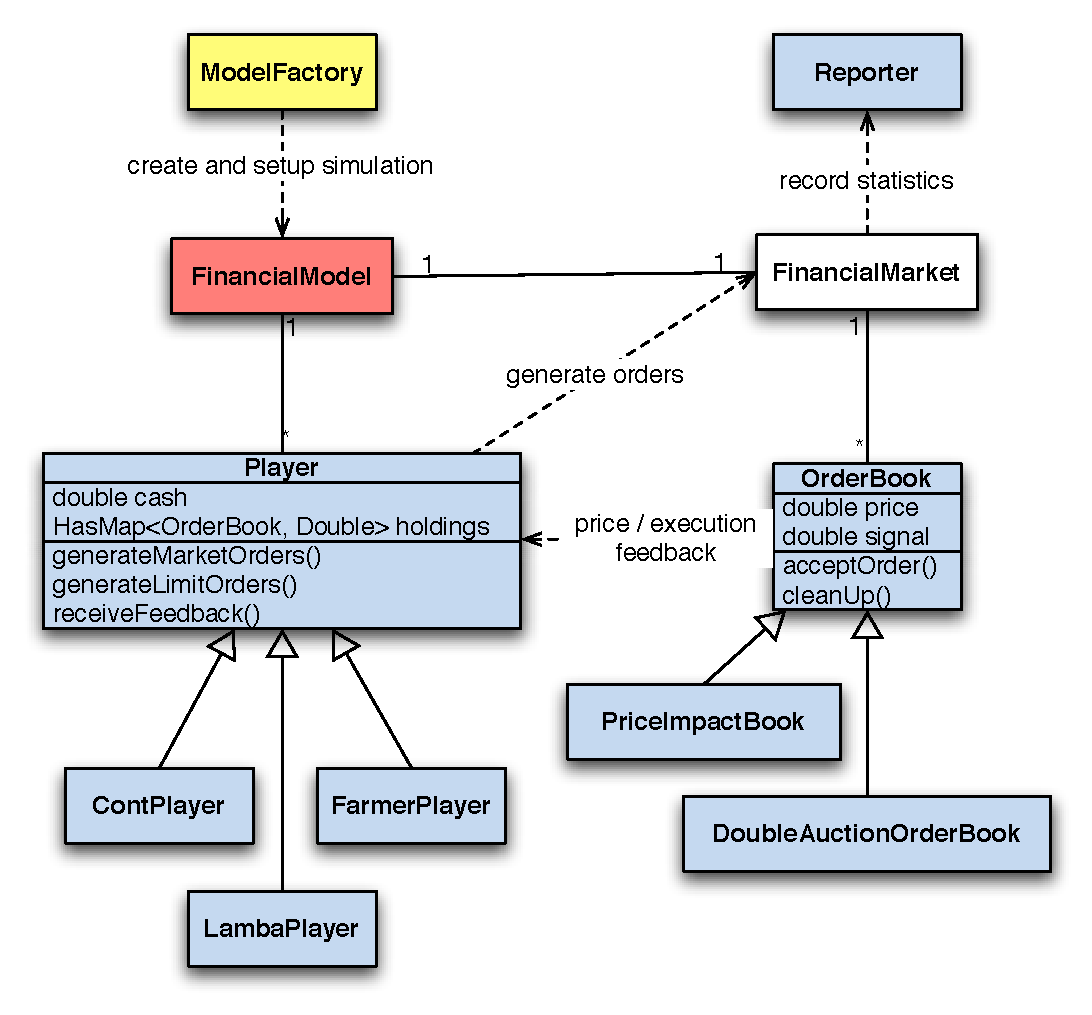
\includegraphics[width=1.0\textwidth]{../graphics/masterClassDiagram.pdf}
\caption{High-level UML class diagram of the main components and relations in the FinancialMarketModel, including the main attributes of Players and OrderBooks. Agent classes (light blue) inherit from the MASON \texttt{Steppable} interface while the master class is implementation of MASON's \texttt{SimState}.}
\label{fig:general_class}
\end{figure}

\begin{figure}[htb]
\centering
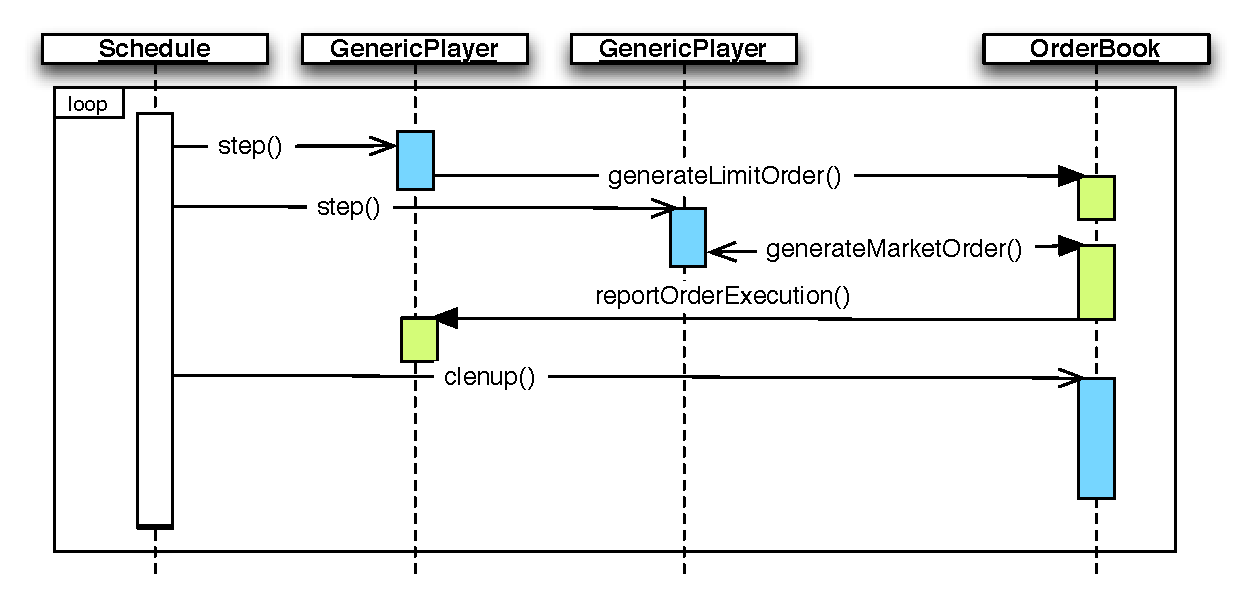
\includegraphics[width=1.0\textwidth]{../graphics/masterSequenceDiagram.pdf}
\caption{High-level UML sequence diagram of the interactions between main object of the FinancialMarketModel, with messages send between two agents and a single orderbook during a single tick shown. Agents are activated by MASON simulation engine and may generate different kinds of \texttt{Market}- and \texttt{LimitOrders}, depending on their internal states and signals from environment (prices, news process). The \texttt{MarketOrder} gives an agent instantaneous feedback, whereupon effects of LimitOrder may be delayed in time. The \texttt{cleanup} signal causes the Orderbook to arbitrage all possible trades between \texttt{LimitOrders}, recalculate new prices and returns (if applicable) and remove expired orders.}
\label{fig:general_sequence}
\end{figure}


\section{Implemented Models}

\subsection{Cont Model}

The Cont model (\cite{cont2006}) is the simplest model implemented. All traders (agents) follow the same behavioral rules. They are heterogeneous in the sense that they are given independently assigned (subjective) volatility thresholds $\theta_i(t)$. Each period, all agents receive a common signal, which can be interpreted as public information or "news", in the form of IID Gaussian random variables $\epsilon_t ~ N(0,D^2)$. Each agent $i$ responds to this signal by selling if $\epsilon_t < -\theta_i(t)$, buying if $\epsilon_t > \theta_i(t)$, and otherwise sitting out the period. The market then determines the excess demand and arrives at the market clearing price by means of a market impact function. Lastly, with probability $s$, agents update their threshold to match the absolute value of the return rate for the current period. Somewhat surprisingly, even this very simple "zero intelligence" model of agent behavior yields fairly realistic market movements, as presented in Figures \ref{fig:ContSmallSSim} (for small $s$) and \ref{fig:ContLargeSSim} (for large value of $s$). 

One down side of the Cont model that is not noted in the papers is that there appears to be a great degree of periodic cyclicality in the volatility of the markets. This is especially apparent with higher probability $s$ of updating thresholds. With $s=0.1$, this is readily apparent if you look at the autocorrelation of absolute returns over longer time scales than shown in the paper. This effect can be particularly well seen when averaging over many runs, as on Figure \ref{fig:ContMultiRun}. Holding $s$ constant at $0.1$ and varying $D$, we find the period and amplitude to be predictable.

\begin{figure}[htbp]
  \begin{center}
   \mbox{
    \subfigure[Trade volumes.]{\scalebox{0.33}{ 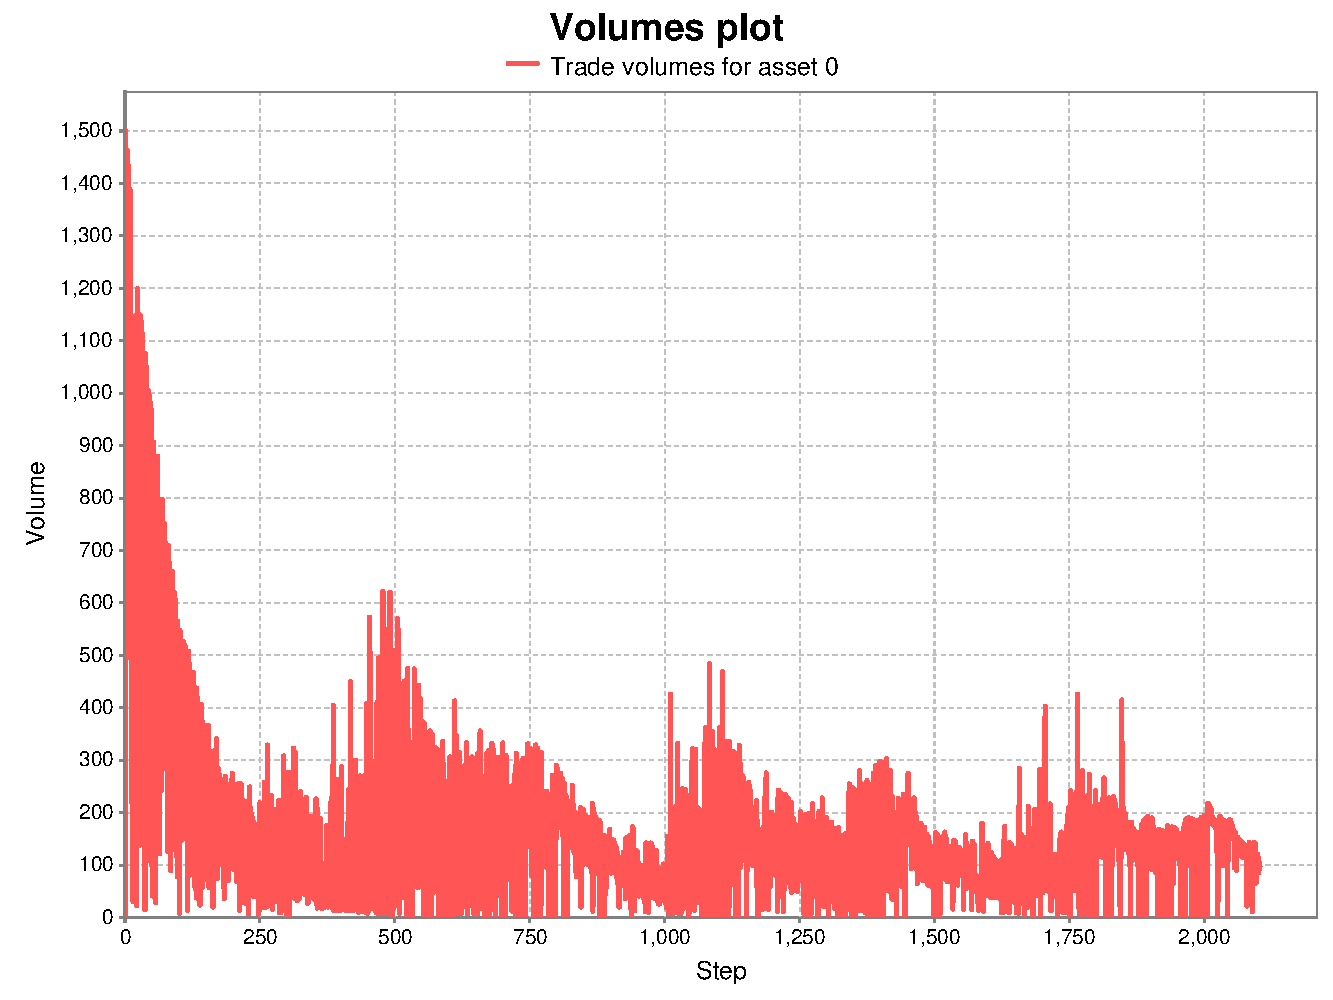
\includegraphics[width=1.00\textwidth]{../graphics/Cont-s01-volumesPlot.pdf}}}
    \quad
\subfigure[Price]{\scalebox{0.33}{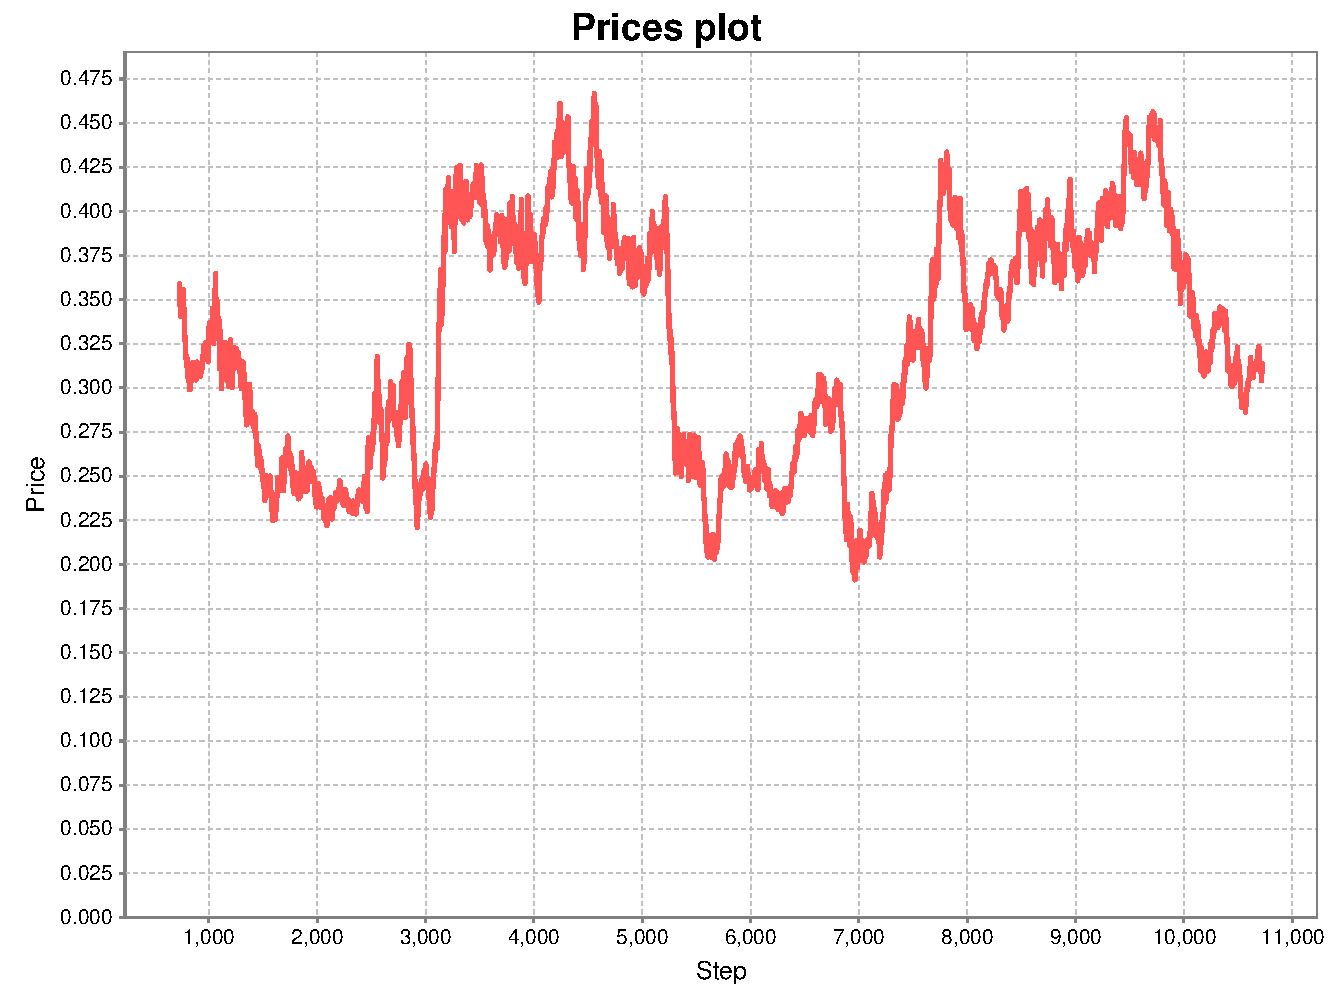
\includegraphics[width=1.0\textwidth]{../graphics/Cont-s01-pricesPlot.pdf}}}
}
    \mbox{
      \subfigure[Raw and absolute returns.]{\scalebox{0.33}{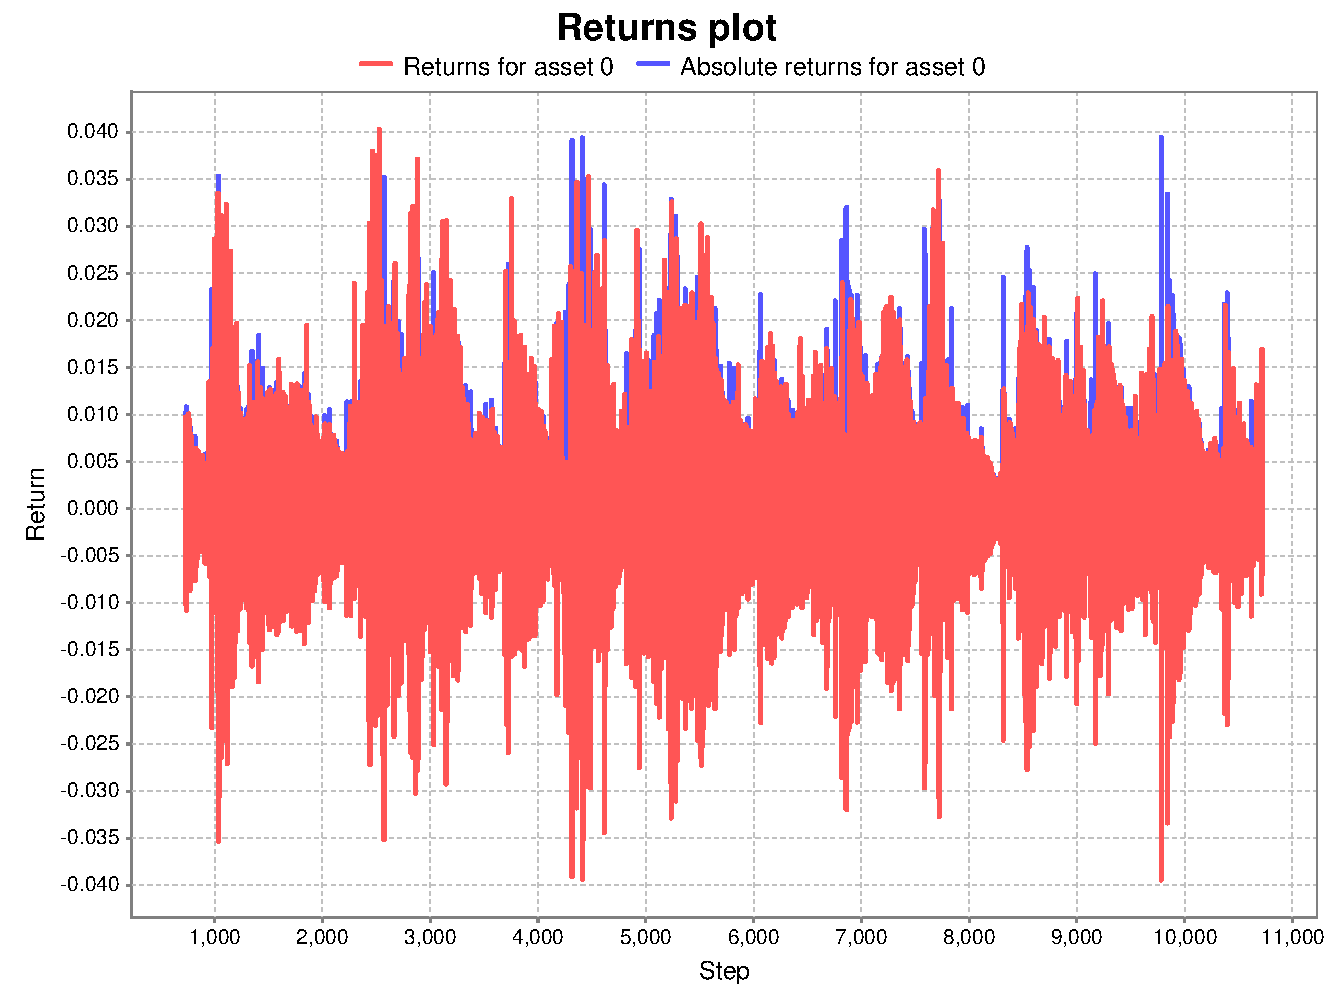
\includegraphics[width=1.00\textwidth]{../graphics/Cont-s01-returnsPlot.pdf}}}
      \quad
      \subfigure[Returns histogram.]{\scalebox{0.33}{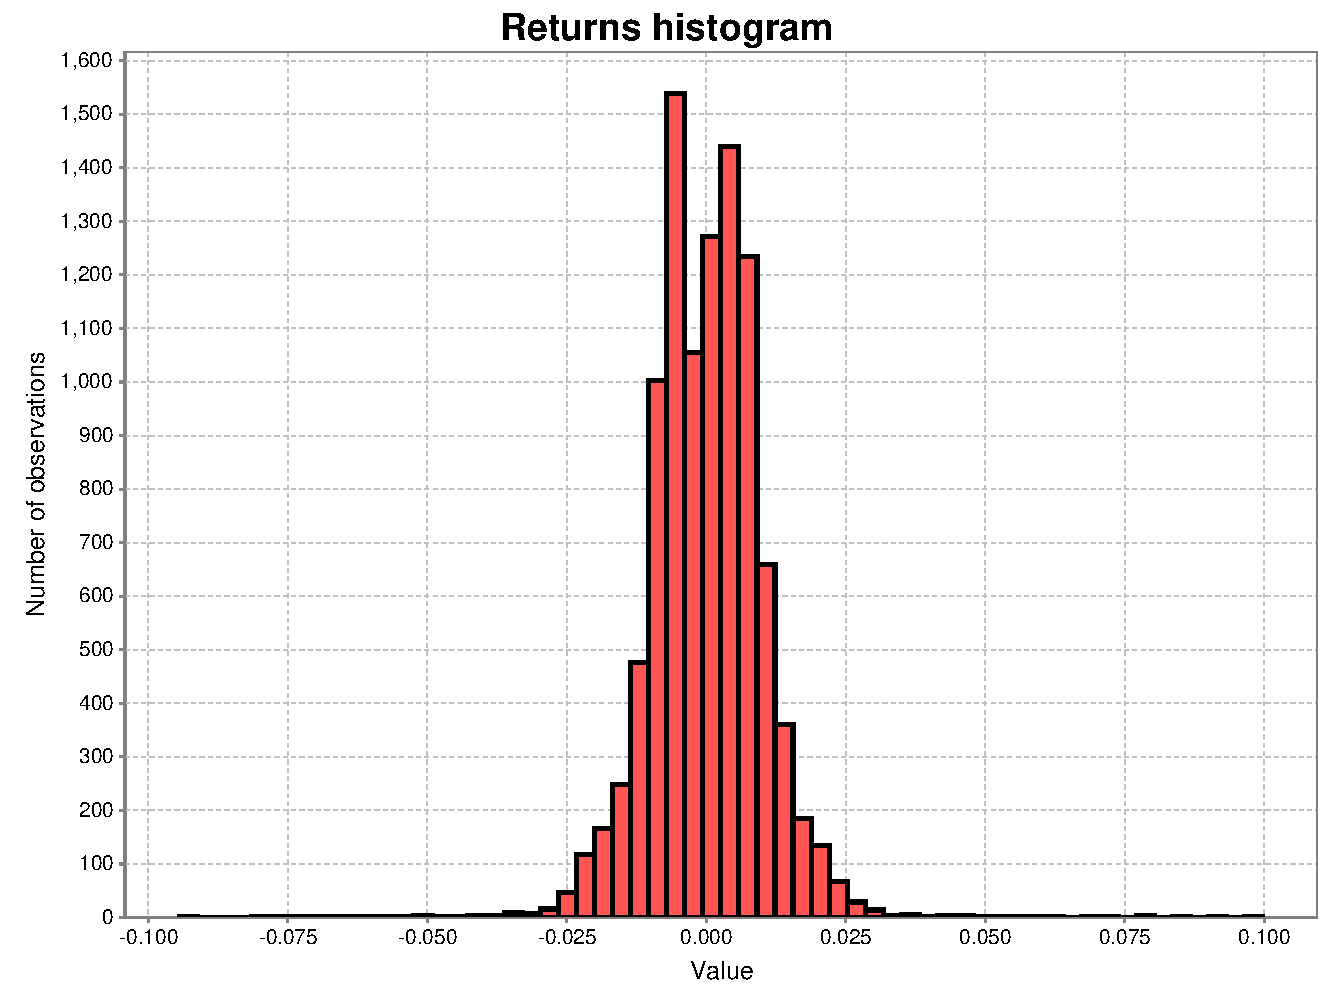
\includegraphics[width=1.00\textwidth]{../graphics/Cont-s01-returnsHistogram.pdf}}}       
      \quad
      \subfigure[Log returns histogram.]{\scalebox{0.33}{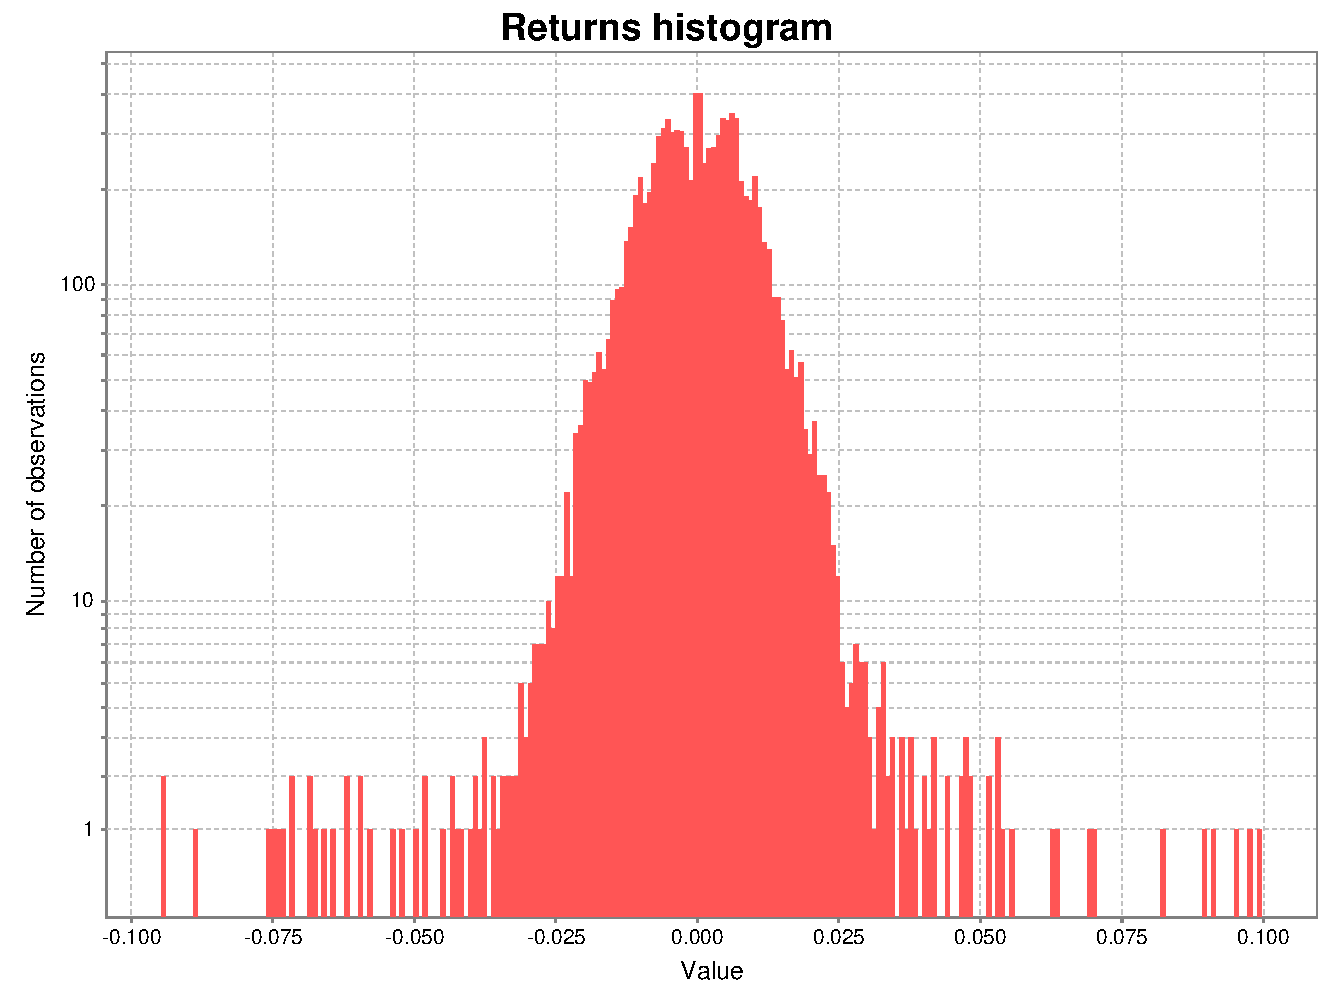
\includegraphics[width=1.00\textwidth]{../graphics/Cont-s01-logReturnsHistogram.pdf}}}       
}
    \mbox{
      \subfigure[Annualized moving average volatility]{\scalebox{0.33}{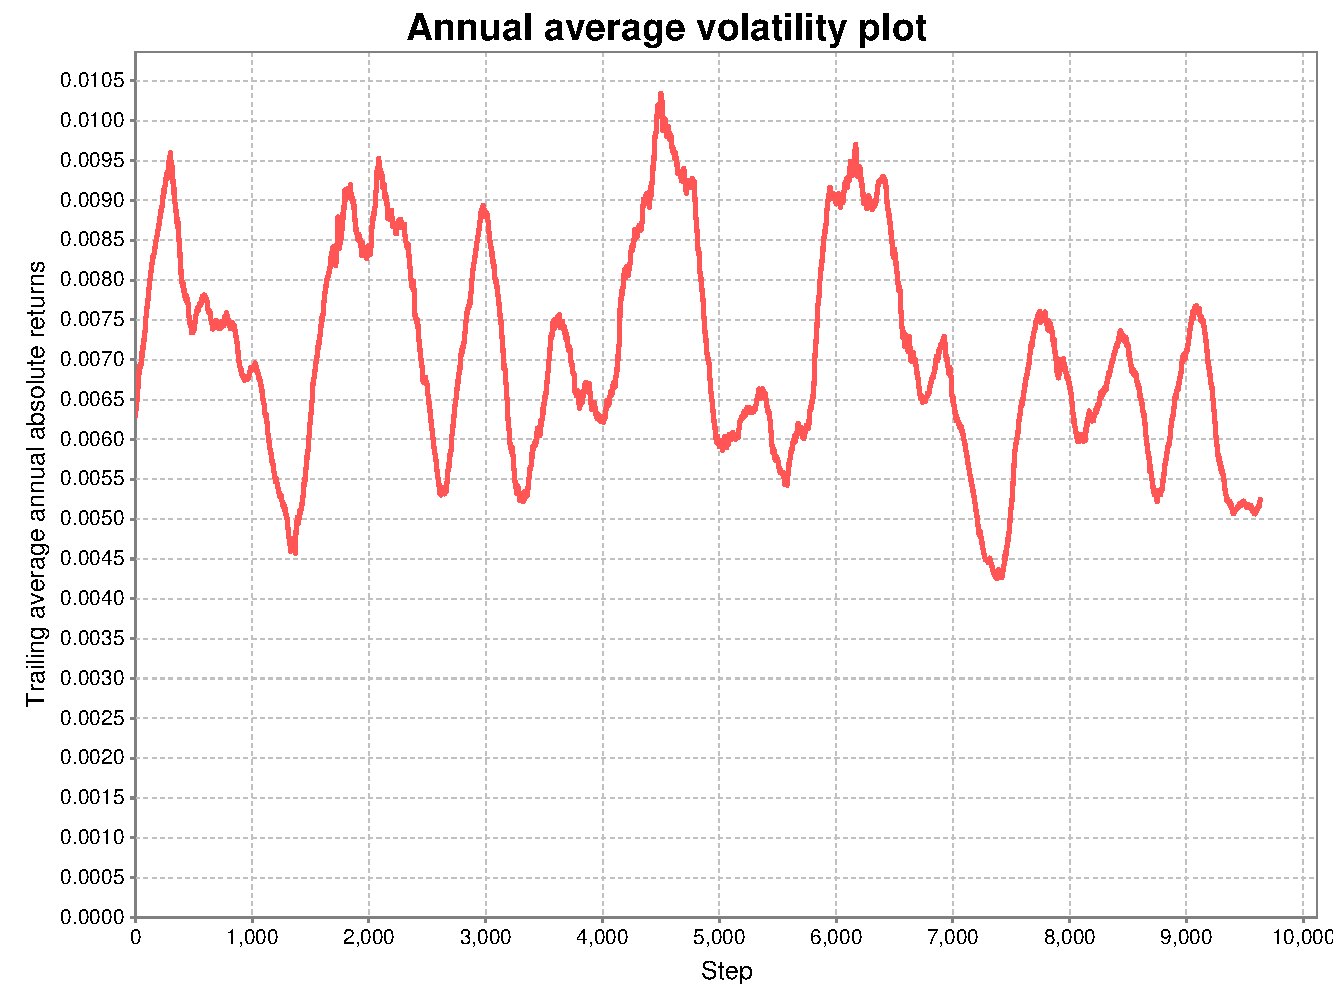
\includegraphics[width=1.00\textwidth]{../graphics/Cont-s01-avgVolatility.pdf}}}
      \quad
      \subfigure[Autocorrelation of returns.]{\scalebox{0.33}{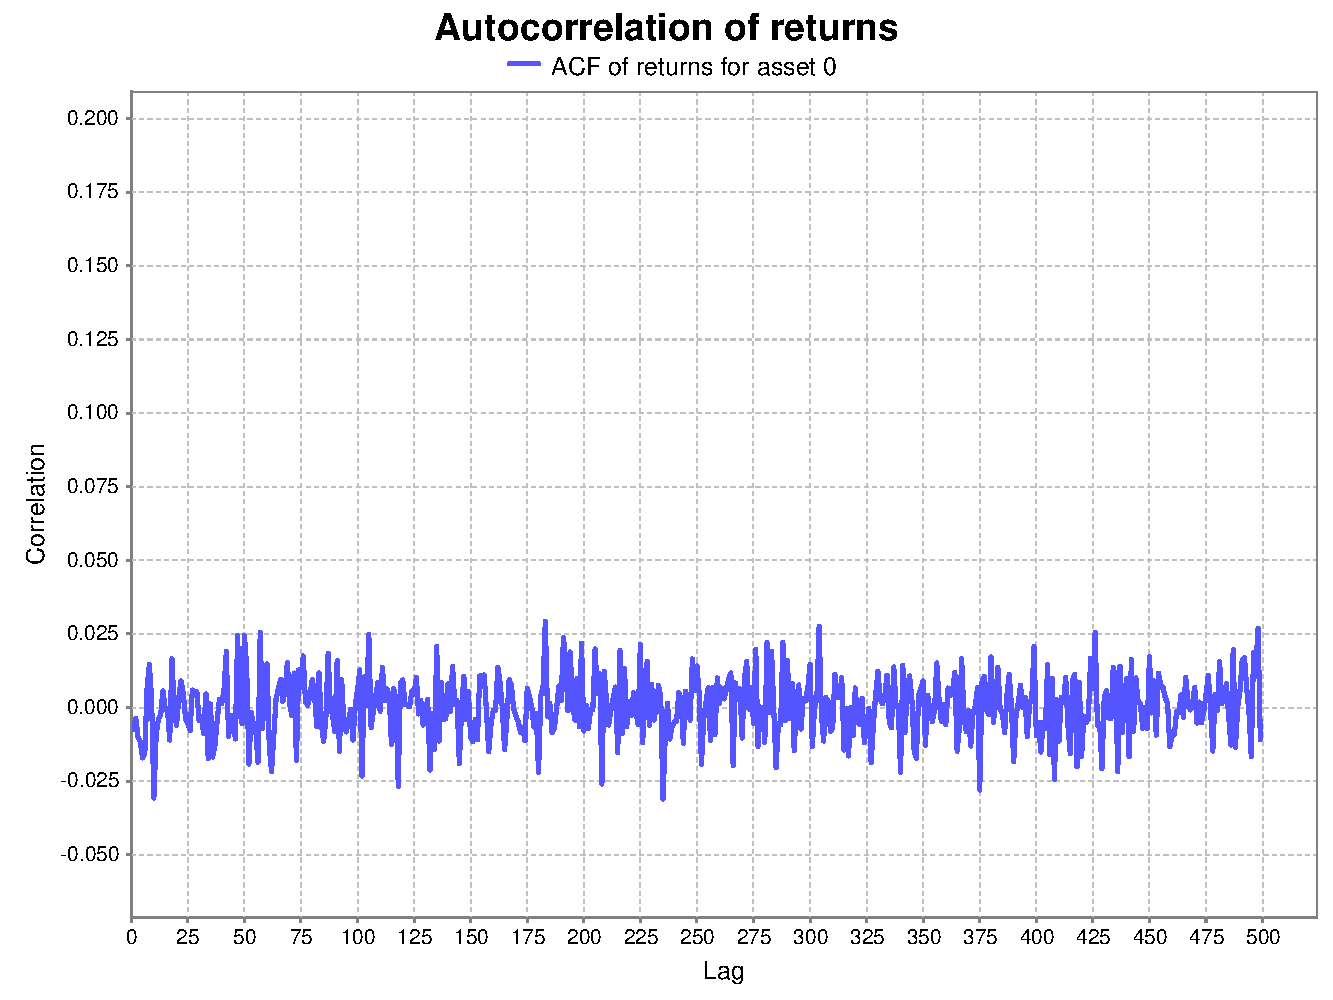
\includegraphics[width=1.00\textwidth]{../graphics/Cont-s01-acfPlot-noAbs.pdf}}}
      \quad
      \subfigure[Autocorrelation of absolute returns.]{\scalebox{0.33}{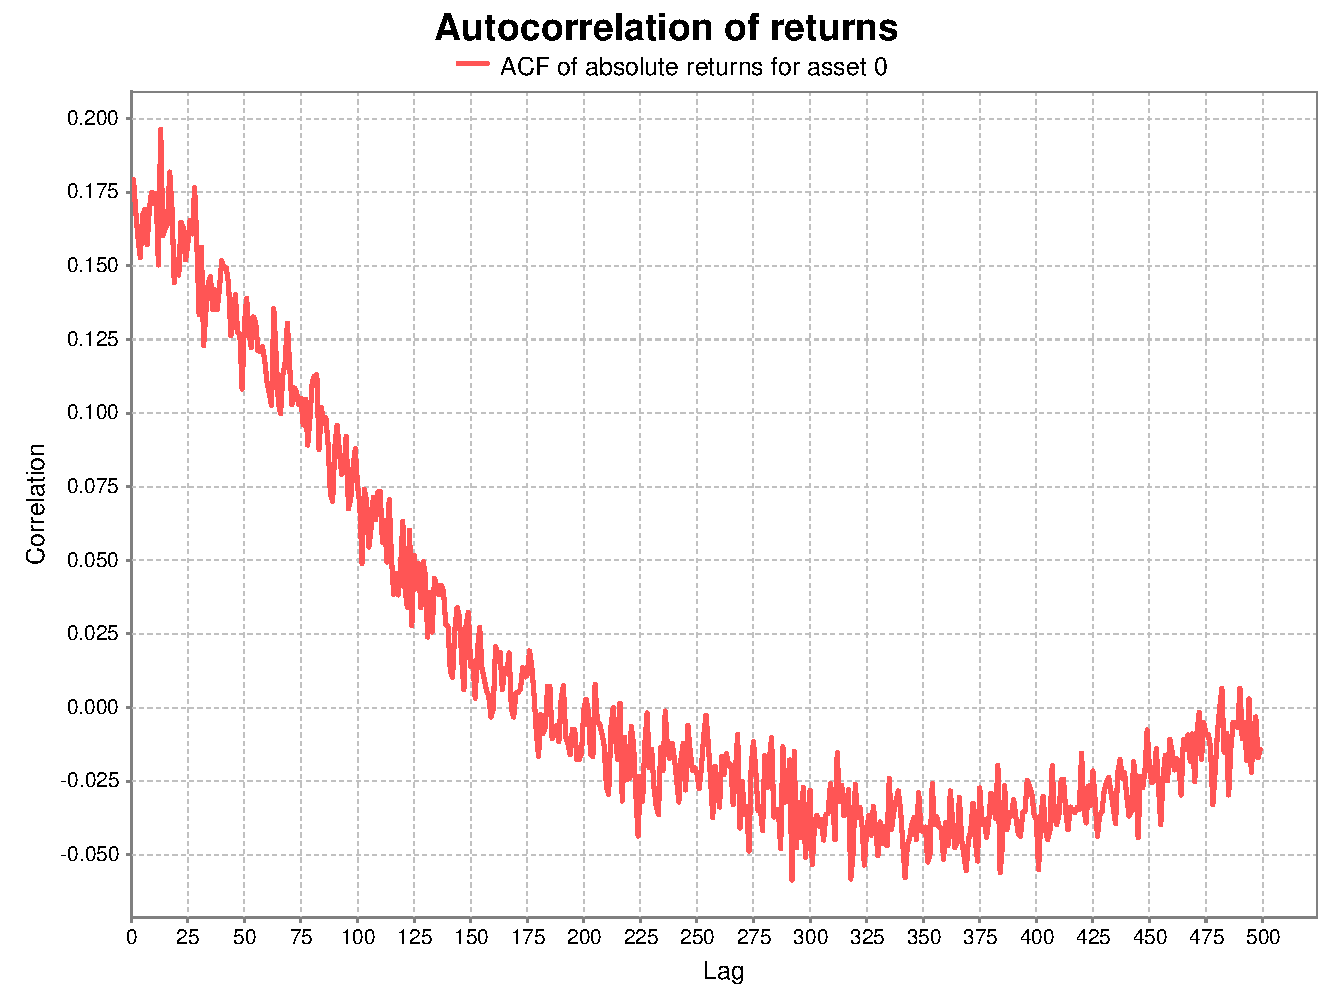
\includegraphics[width=1.00\textwidth]{../graphics/Cont-s01-acfPlot-absonly.pdf}}}
      }
    \caption{Examples of outputs and statistics from a single run of the Cont FinancialModel simulation with $D=0.001$, $s=0.01$.}
    \label{fig:ContSmallSSim}
  \end{center}
\end{figure}




\begin{figure}[htbp]
  \begin{center}
   \mbox{
      \subfigure[Trade volumes.]{\scalebox{0.33}{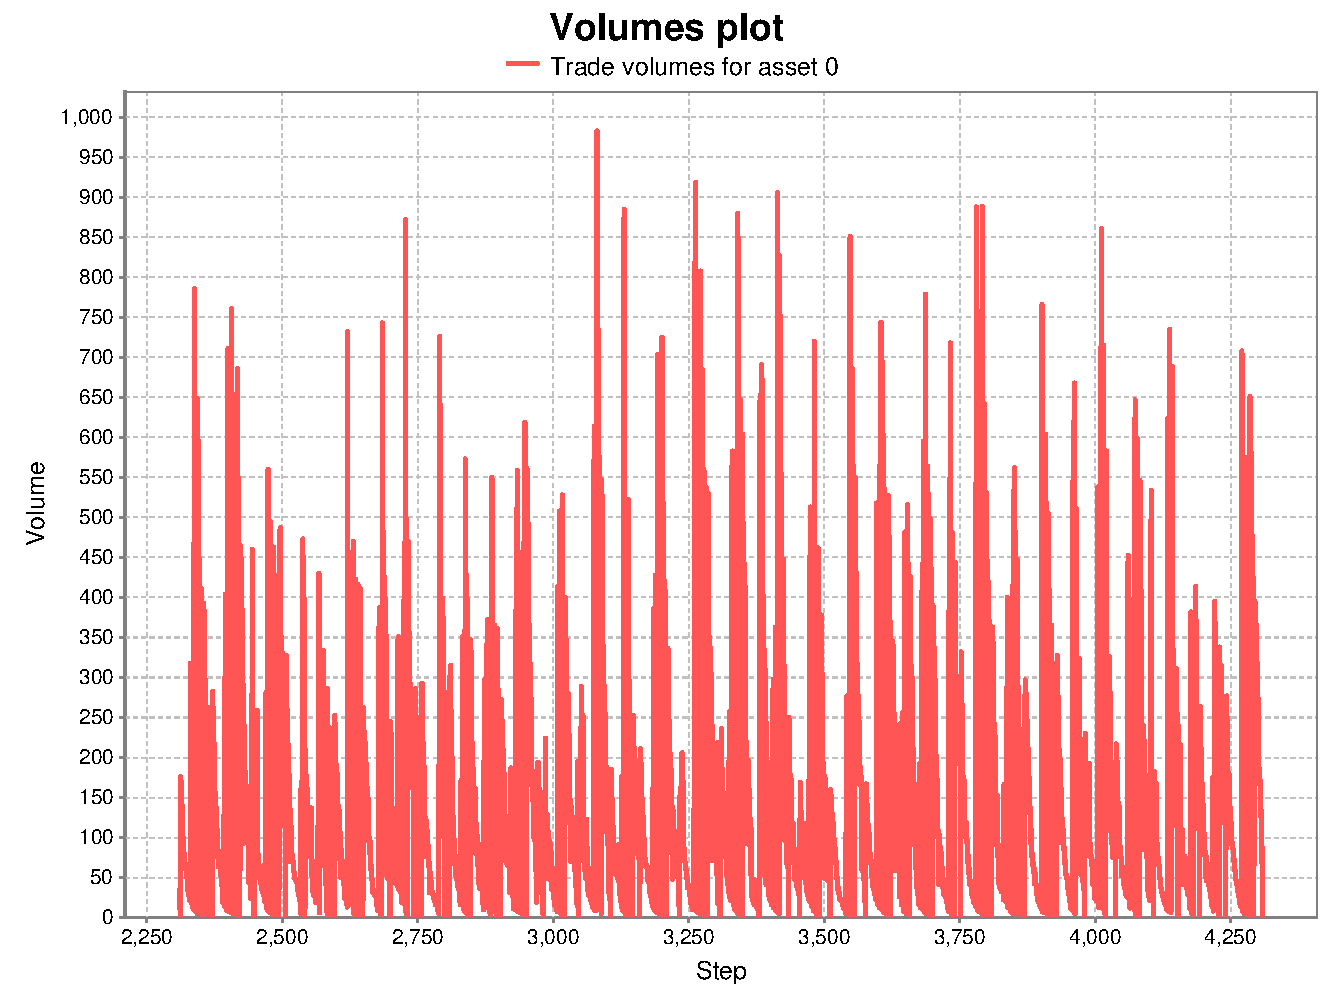
\includegraphics[width=1.00\textwidth]{../graphics/Cont-volumesPlot.pdf}}}
      \quad
      \subfigure[Price]{\scalebox{0.33}{ 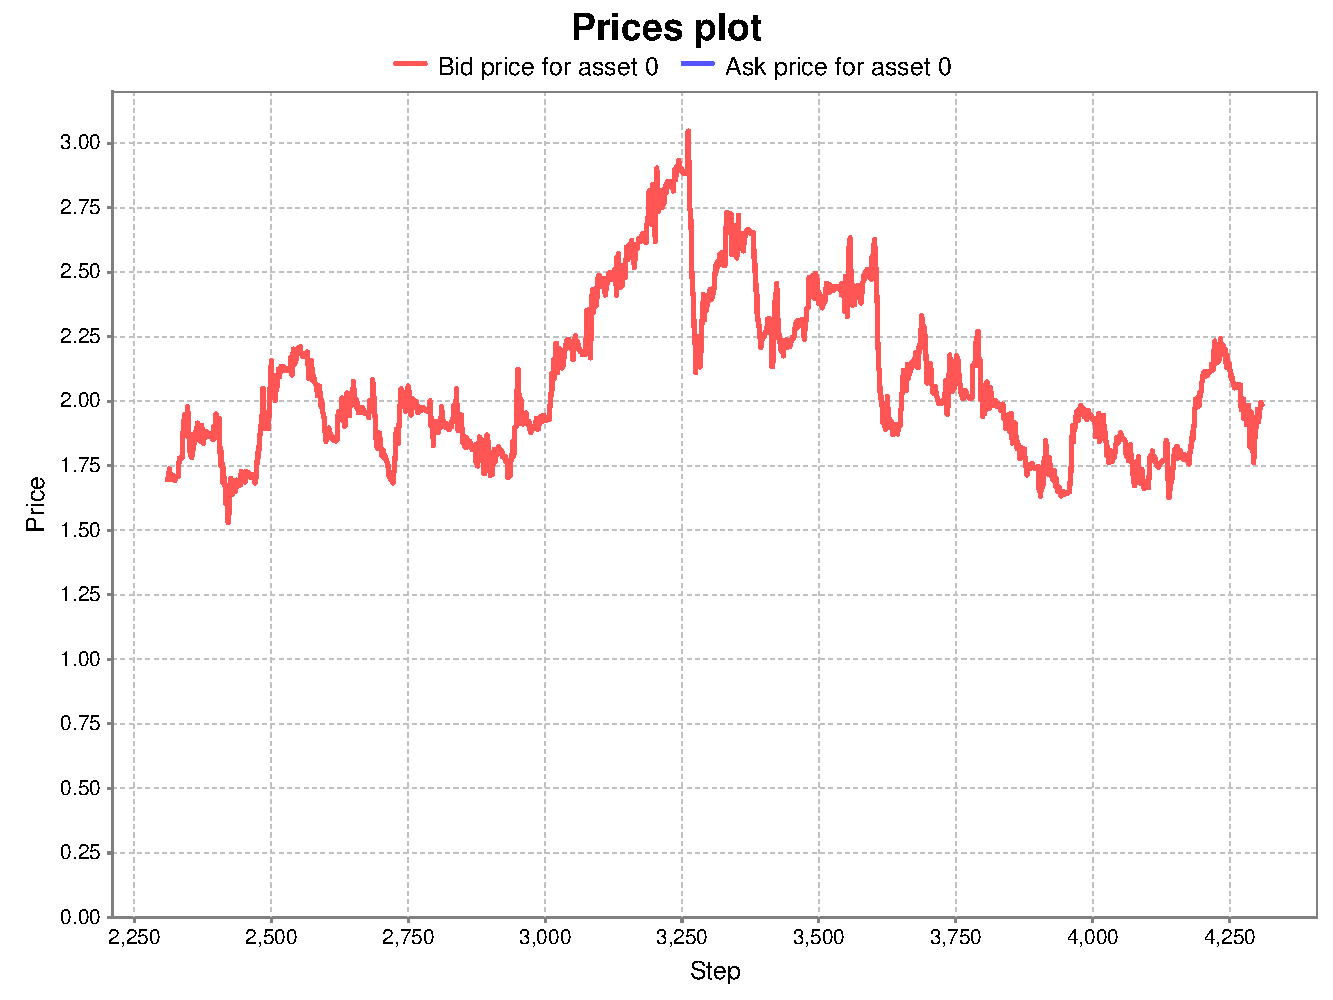
\includegraphics[width=1.0\textwidth]{../graphics/Cont-pricesPlot.pdf}}} \quad
      }
    \mbox{
      \subfigure[Raw and absolute log returns.]{\scalebox{0.33}{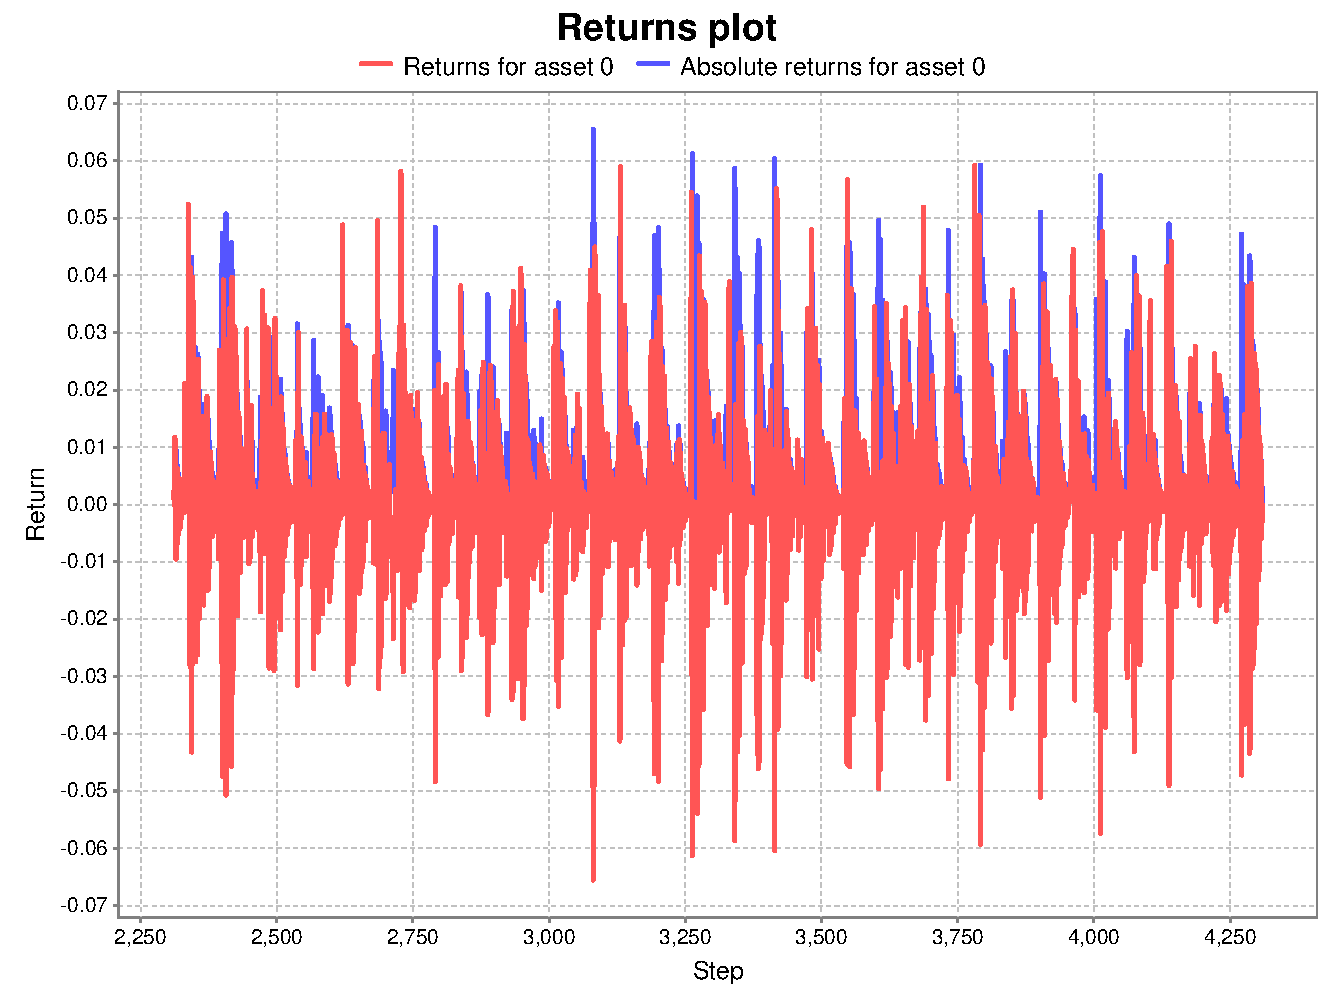
\includegraphics[width=1.00\textwidth]{../graphics/Cont-returnsPlot.pdf}}}
      \quad
      \subfigure[Returns histogram.]{\scalebox{0.33}{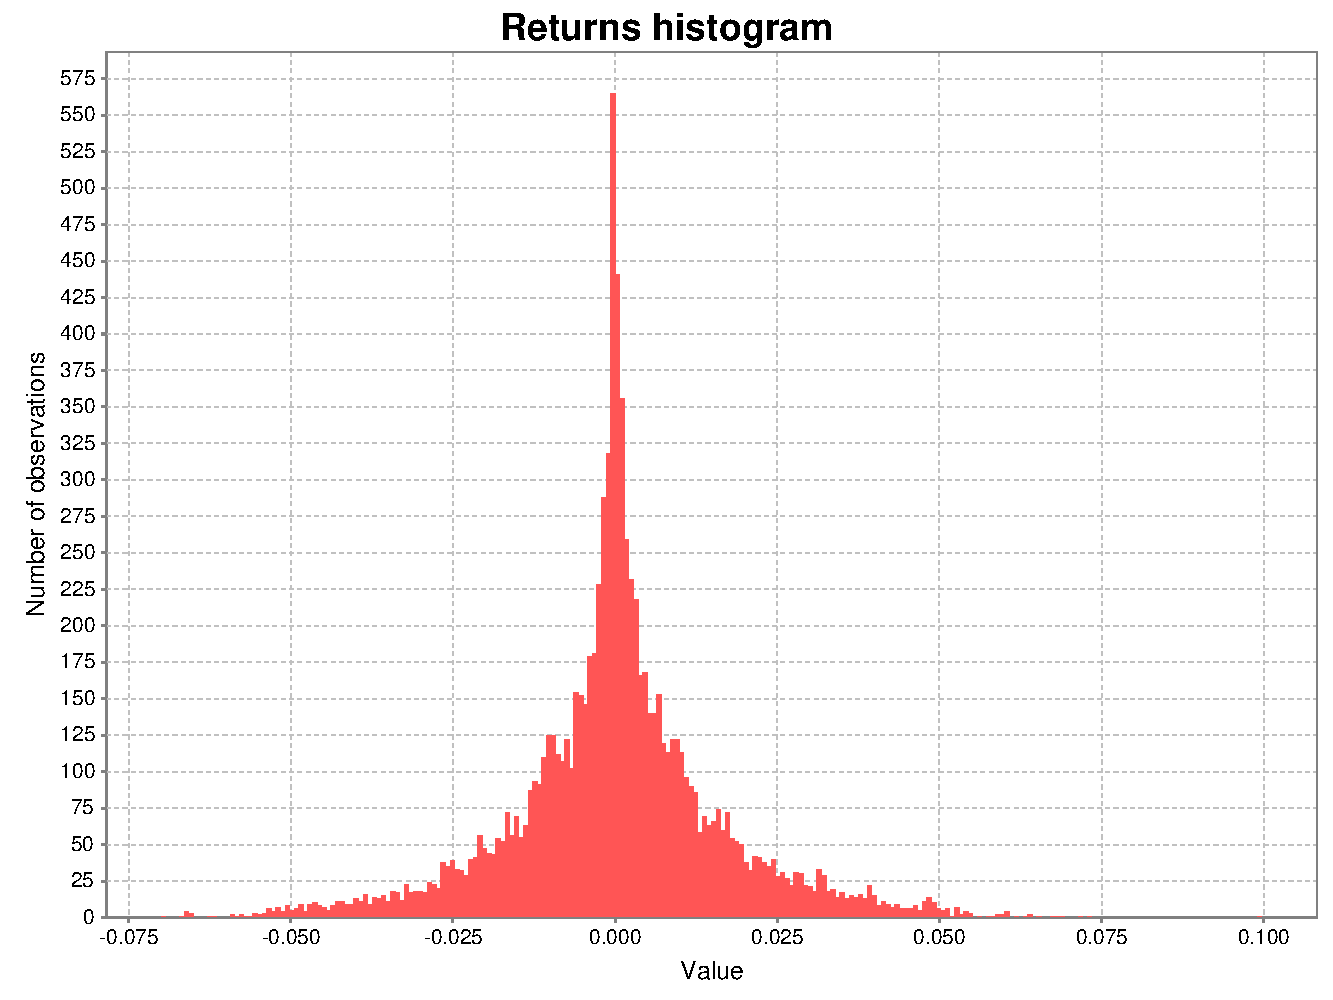
\includegraphics[width=1.00\textwidth]{../graphics/Cont-returnsHistogram.pdf}}}
      \quad
      \subfigure[Log returns histogram.]{\scalebox{0.33}{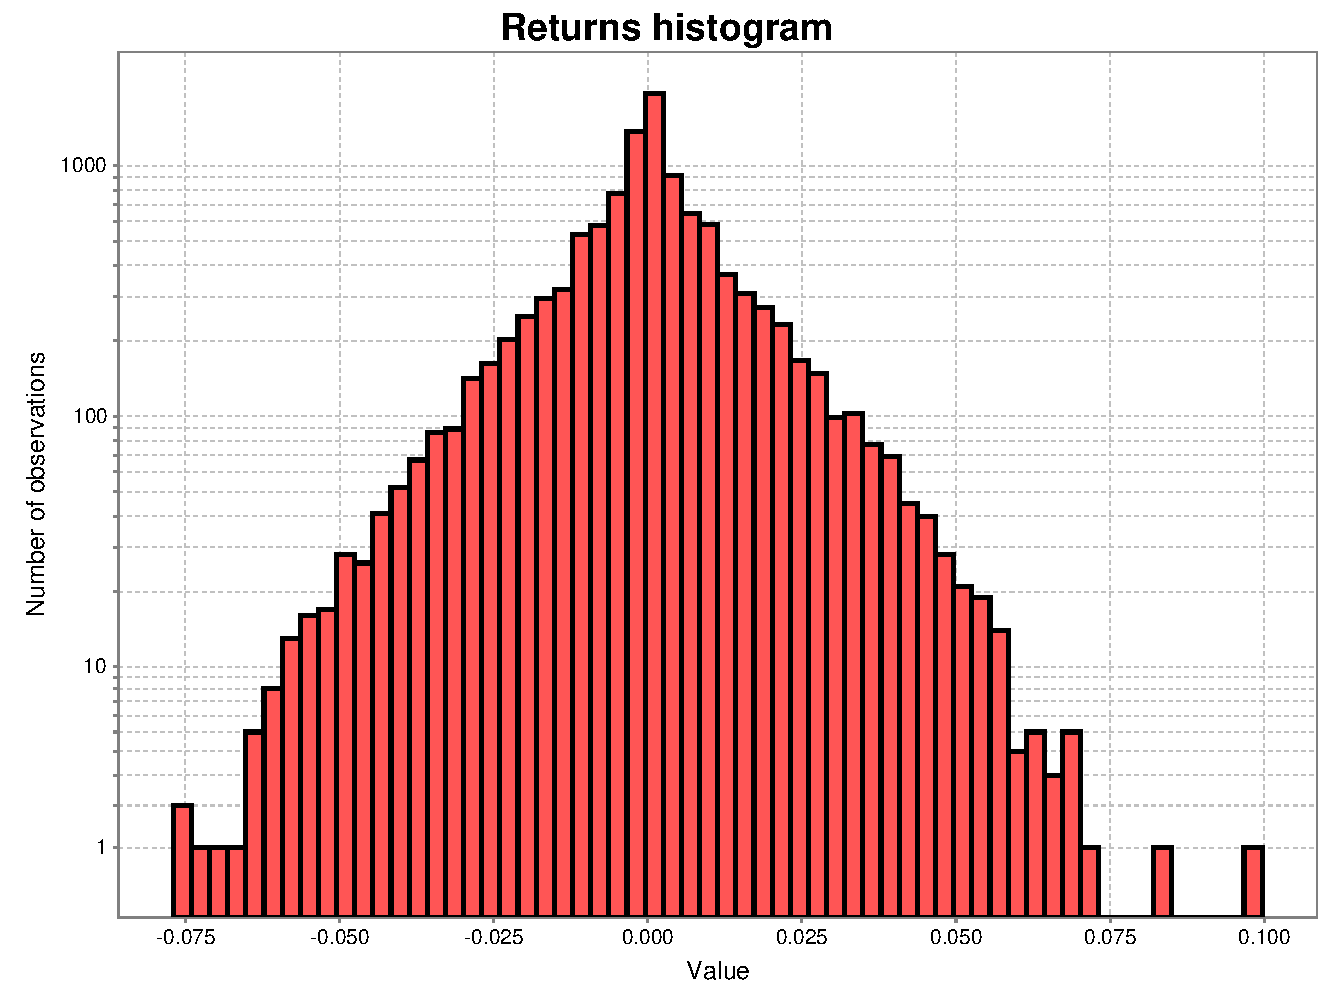
\includegraphics[width=1.00\textwidth]{../graphics/Cont-logReturnsHistogram.pdf}}}       
}
    \mbox{
      \subfigure[Annualized moving average volatility]{\scalebox{0.33}{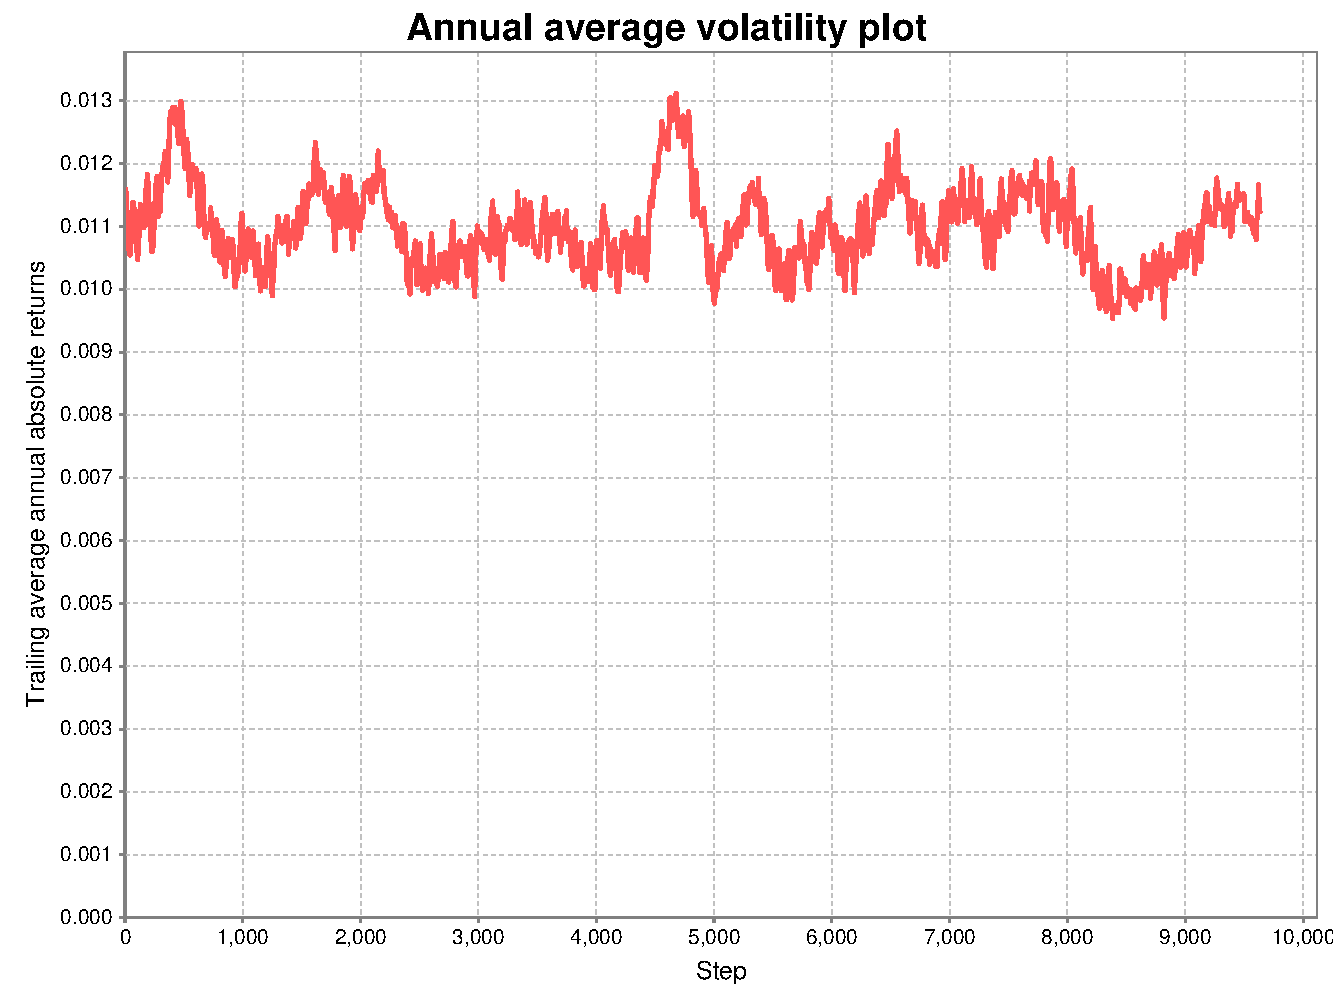
\includegraphics[width=1.00\textwidth]{../graphics/Cont-avgVolatility.pdf}}}
      \quad
      \subfigure[Autocorrelation of returns.]{\scalebox{0.33}{\includegraphics[width=1.00\textwidth]{../graphics/Cont-acfPlot-noAbs.pdf}}}
      \quad
      \subfigure[Autocorrelation of absolute returns.]{\scalebox{0.33}{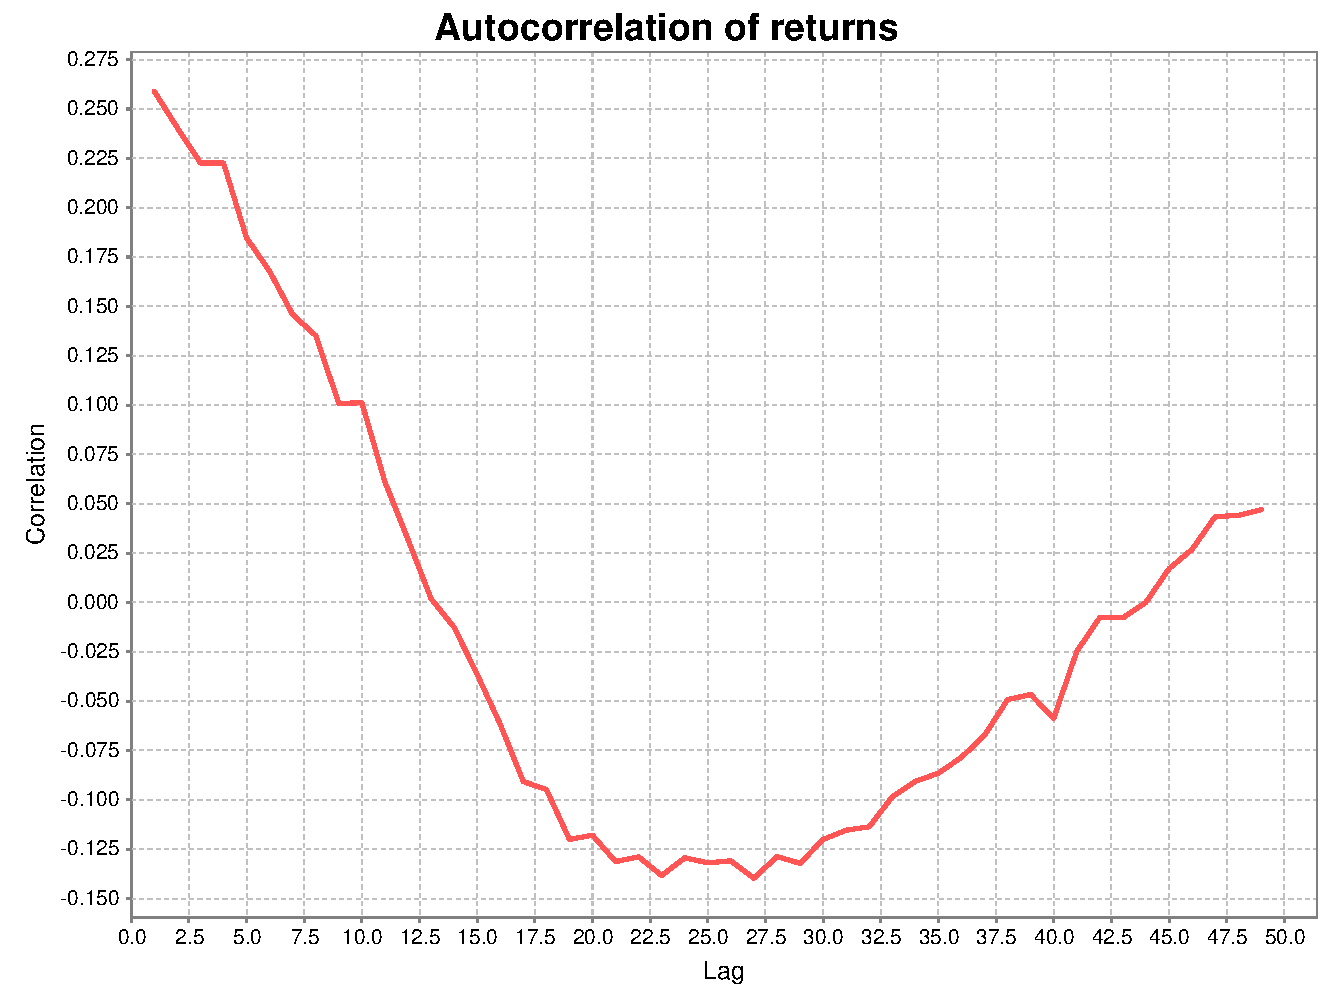
\includegraphics[width=1.00\textwidth]{../graphics/Cont-acfPlot-absonly-to50.pdf}}}
      }
    \caption{Examples of outputs and statistics from a single run of the Cont FinancialModel simulation with $D=0.001$, $s=0.1$.}
    \label{fig:ContLargeSSim}
  \end{center}
\end{figure}


\subsection{Farmer Model}

The Farmer model (\cite{farmer2003}) has two types of agents, which trade a single asset by means of a continuous double auction similar to those normally used on stock markets. "Patient" traders place limit orders, which specify both a price and quantity they wish to buy or sell. Limit orders do not execute immediately, and may be canceled at any time. "Impatient" traders place market orders, specifying only a quantity, which execute immediately at the current best price, assuming there is sufficient liquidity provided by outstanding limit orders. This model also has simple behavioral logic for traders. Behavior is regulated by:
\begin{itemize}
\item Patient agents place \texttt{LimitOrders} of constant size at a Poisson rate per unit time, and with a randomly generated price. Orders are equally likely to be either buy or sell orders. Buy limit orders are placed uniformly anywhere in the semiinfinite interval below the current ask price ($-\infty < p < a(t)$), where $p$ is the \emph{logarithm} of the price; similarly for sell orders. A uniform distribution in log prices is equivalent to an exponential distribution in prices. In addition, outstanding limit orders are canceled at a Poisson rate per unit time. All of these processes are independent.
\item Impatient agents place \texttt{MarketOrders} of constant size at a certain Poisson rate per unit time.
\item A double auction order book. This manages the pending limit orders and facilitates trades between market and limit orders. It also provides aggregate market information such as return rate per unit time and bid-ask spreads.
\end{itemize}
This model explains a large portion of the spread and price diffusion of actual stocks given an order flow rate, which essentially means that the double auction structure has a large impact on the nature of market movements. The model also yields market behavior qualitatively close to actual markets in many respects, see Figure \ref{fig:sampleDynamicsFarmer}.

\begin{figure}[htbp]
  \begin{center}
   \mbox{
      \subfigure[Ask and bid prices.]{\scalebox{0.5}{\quad \quad 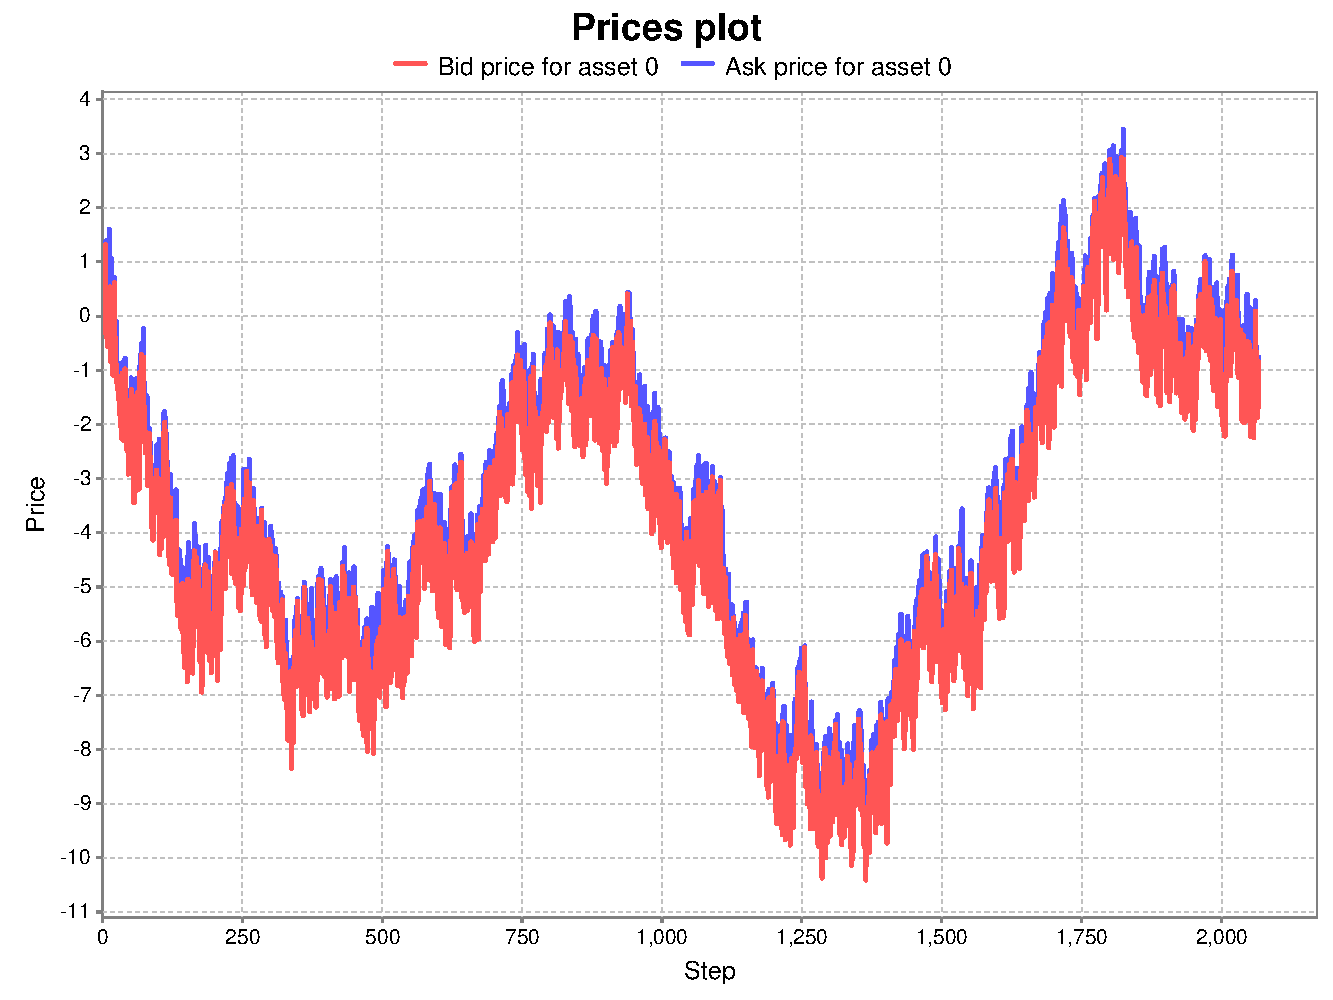
\includegraphics[width=1.0\textwidth]{../graphics/Farmer-pricesPlot.pdf}}} \quad
      \subfigure[Raw and absolute returns.]{\scalebox{0.5}{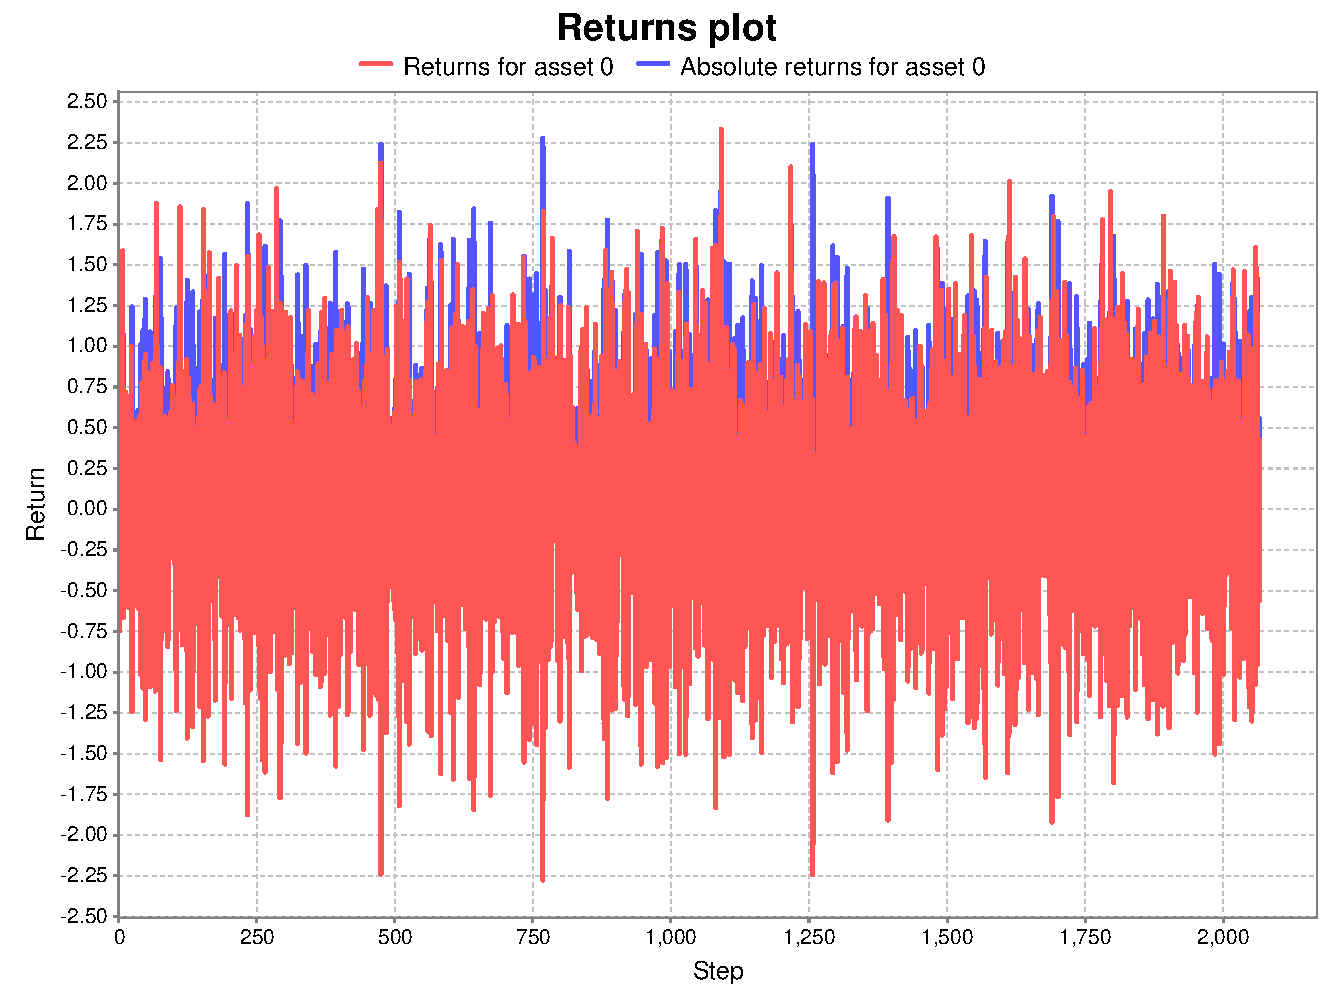
\includegraphics[width=1.00\textwidth]{../graphics/Farmer-returnPlot.pdf}}}
      }
    \mbox{
      \subfigure[Orderbook shape.]{\scalebox{0.5}{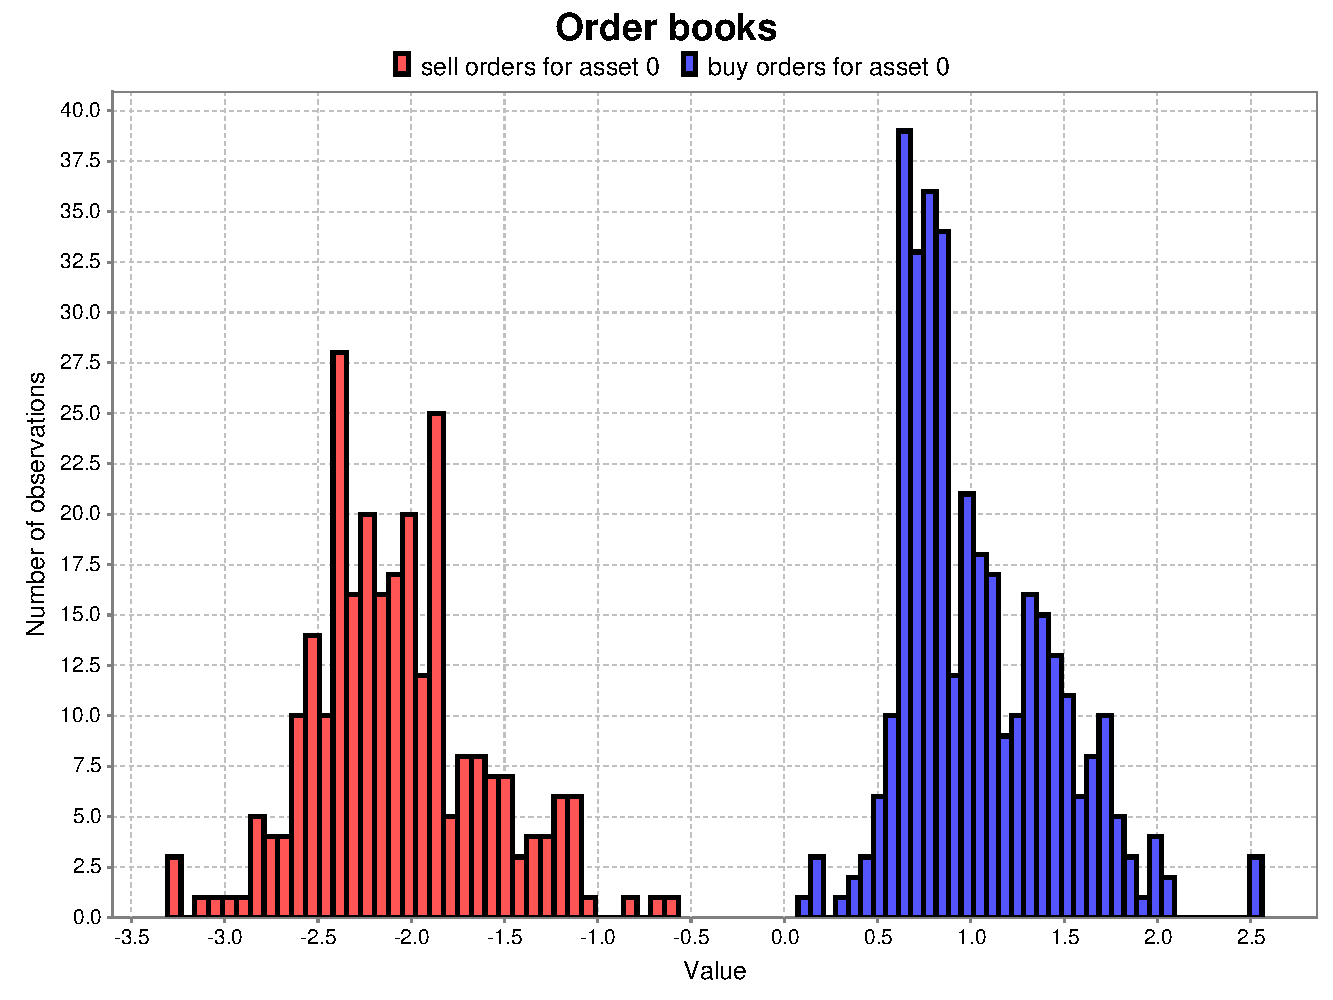
\includegraphics[width=1.00\textwidth]{../graphics/Farmer-orderbooks.pdf}}} \quad
      \subfigure[Trade volumes.]{\scalebox{0.5}{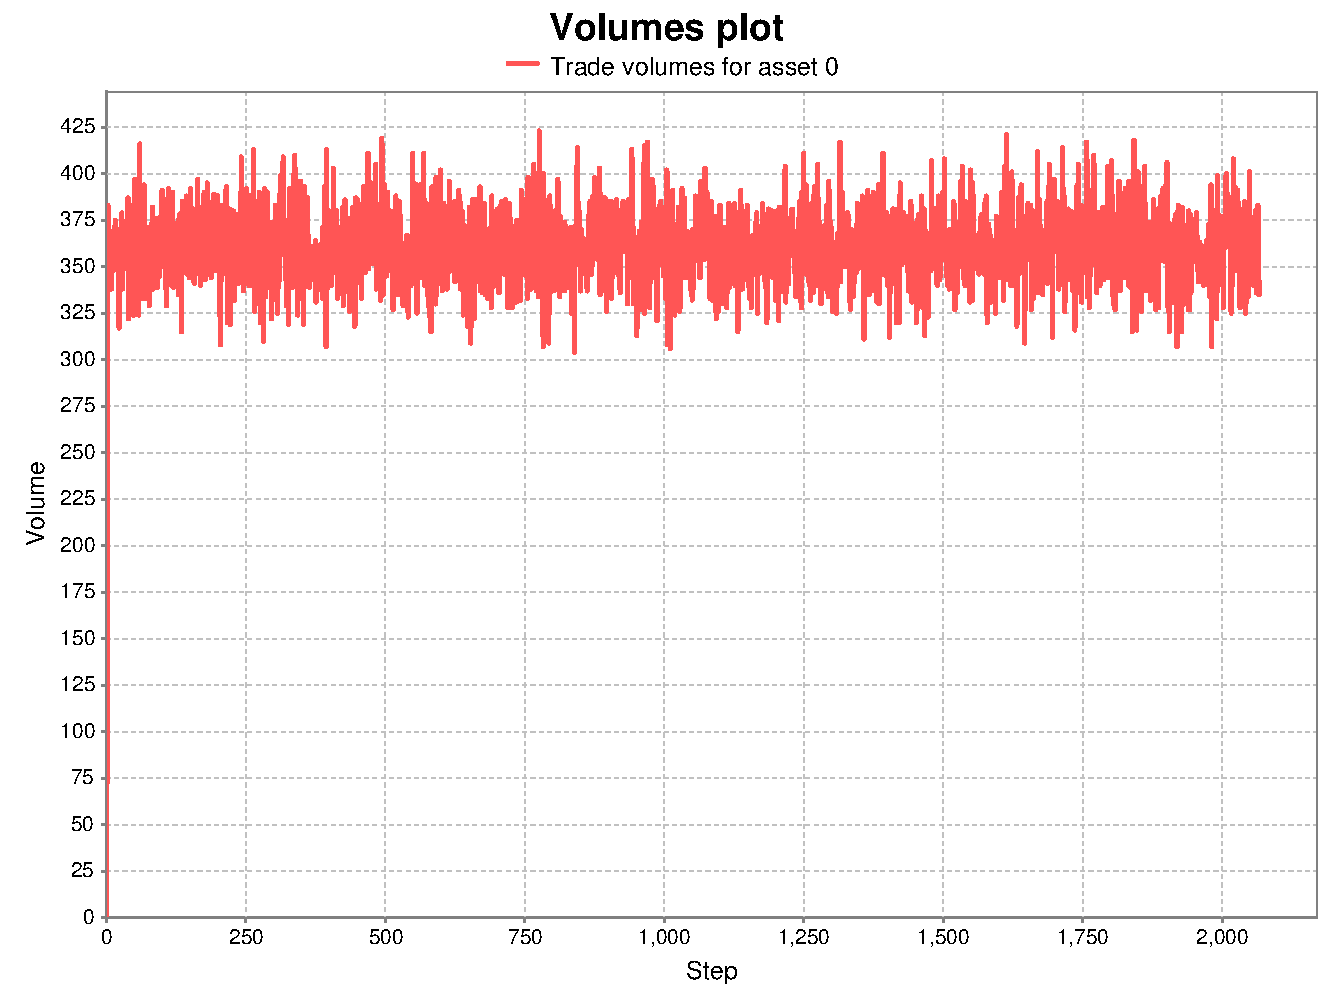
\includegraphics[width=1.00\textwidth]{../graphics/Farmer-volumesPlot.pdf}}}
      }
    \mbox{
      \subfigure[Returns histogram.]{\scalebox{0.5}{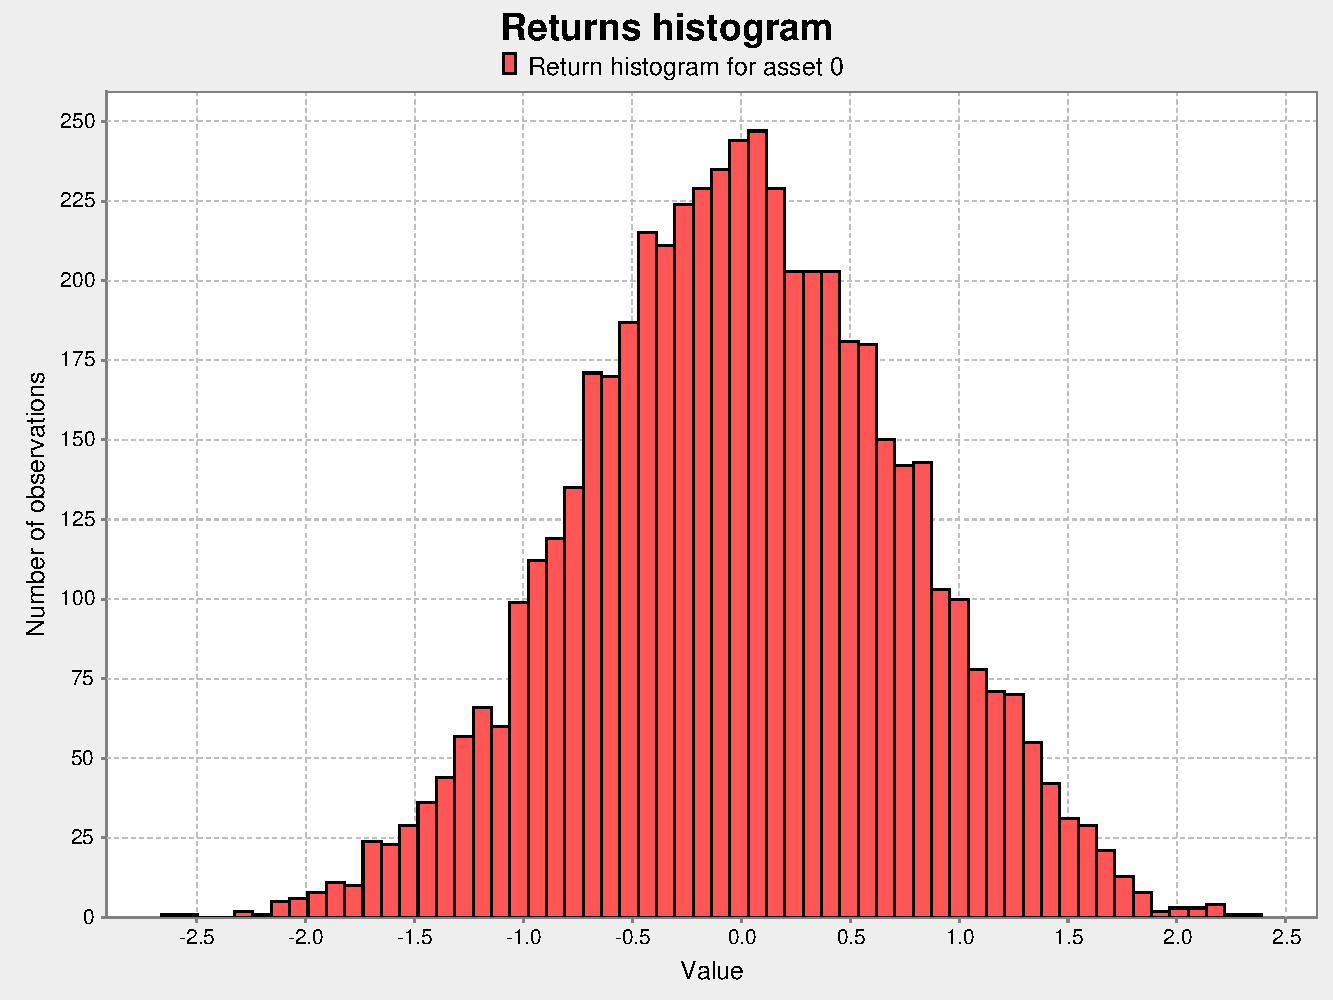
\includegraphics[width=1.00\textwidth]{../graphics/Farmer-returnsHistogram.pdf}}} \quad
      \subfigure[Autocorrelation of returns.]{\scalebox{0.5}{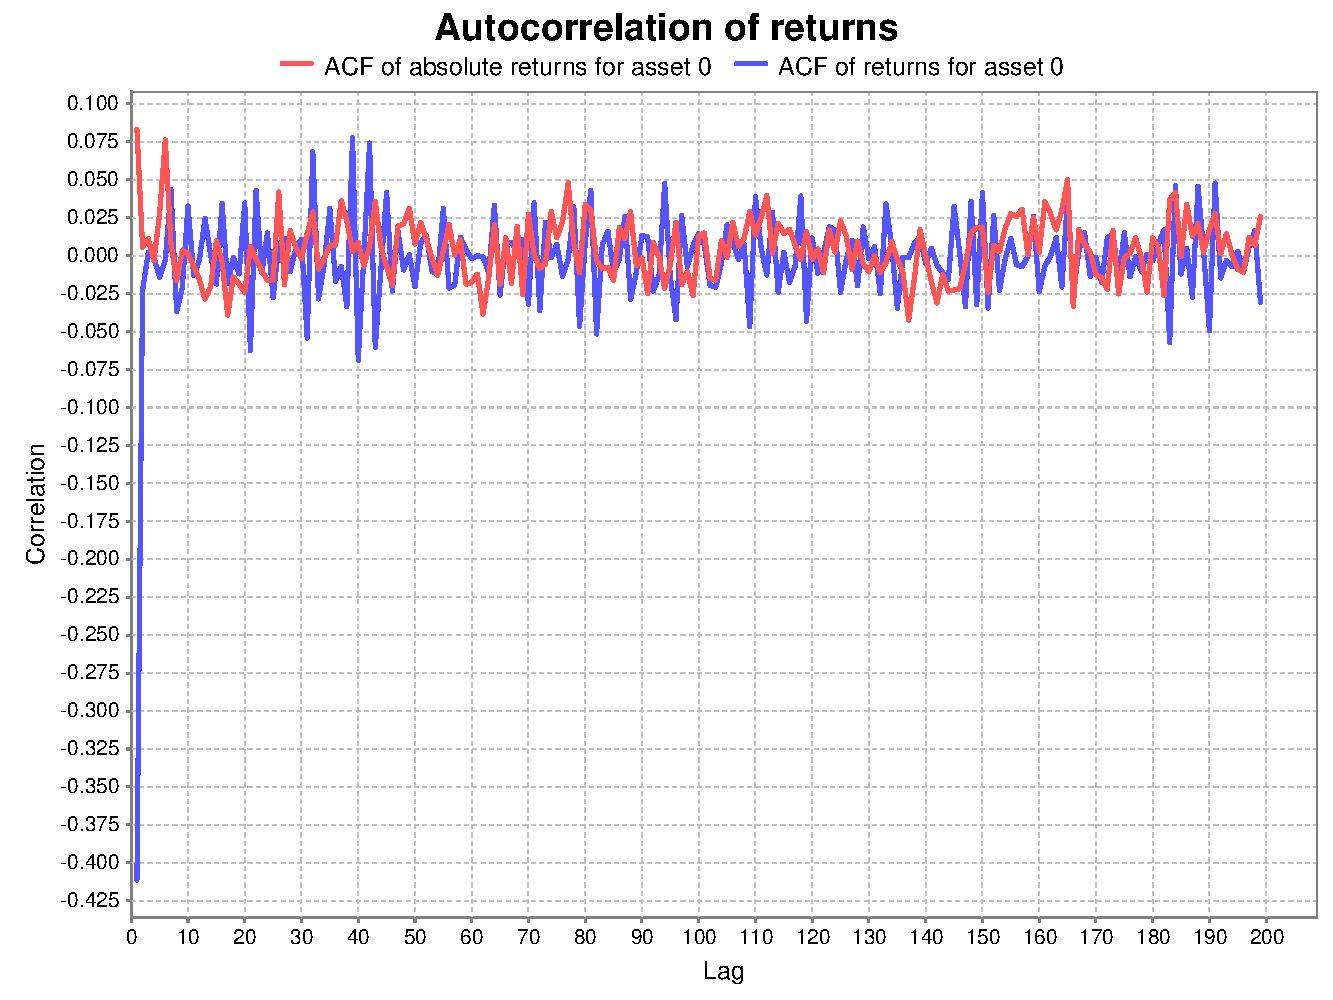
\includegraphics[width=1.00\textwidth]{../graphics/Farmer-acfReturns.pdf}}}
      }
    \caption{Examples of outputs and statistics from a single run of the FinancialModel simulation for default Farmer's parametrization.}
    \label{fig:sampleDynamicsFarmer}
  \end{center}
\end{figure}

\subsection{Farmer-Cont Model}

As an experiment, we constructed a model combining some aspects of the Farmer model with some aspects of the Cont model. The result is a model which is still essentially zero intelligence, but which exhibits empirically positive characteristics of both models. In this model there are two types of agents, which interact via the continuous double auction mechanism, as in Farmer. In fact, the Patient traders, which place limit orders and thus provide liquidity, remain the same. Impatient traders are modeled after Cont. They have heterogeneous volatility thresholds, and place market orders depending upon how public information in the form of a normally distributed random variable compares with these thresholds. Some fraction $s$ of agents then adjust their volatility thresholds in light of current volatility by setting it to the trailing period's return rate.

\begin{figure}[htbp]
  \begin{center}
   \mbox{
      \subfigure[Trade volumes.]{\scalebox{0.33}{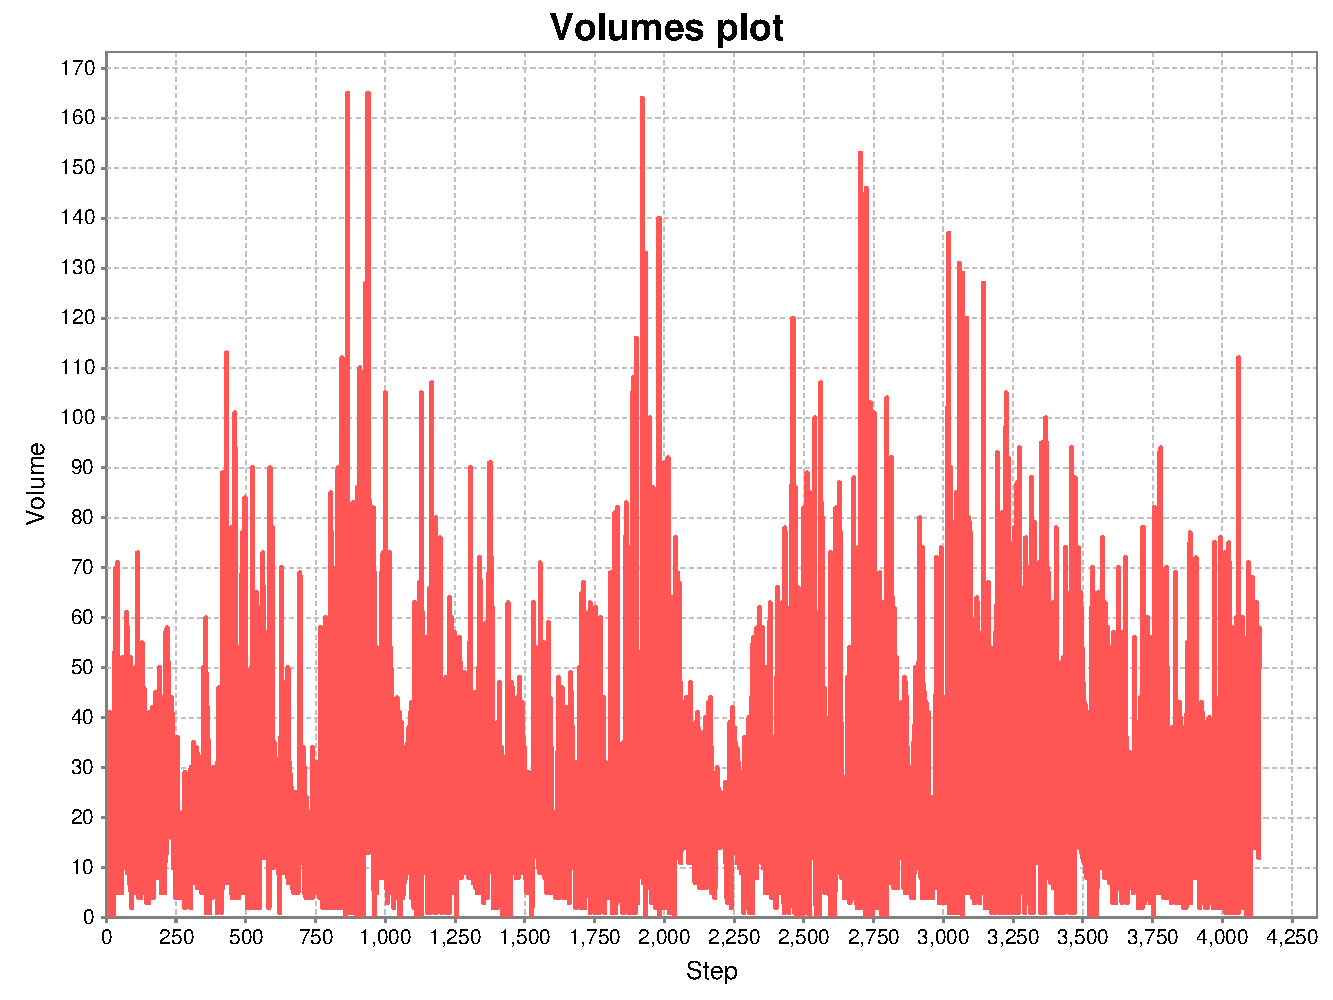
\includegraphics[width=1.00\textwidth]{../graphics/FC-volumesPlot.pdf}}}
      \quad
      \subfigure[Price]{\scalebox{0.33}{ 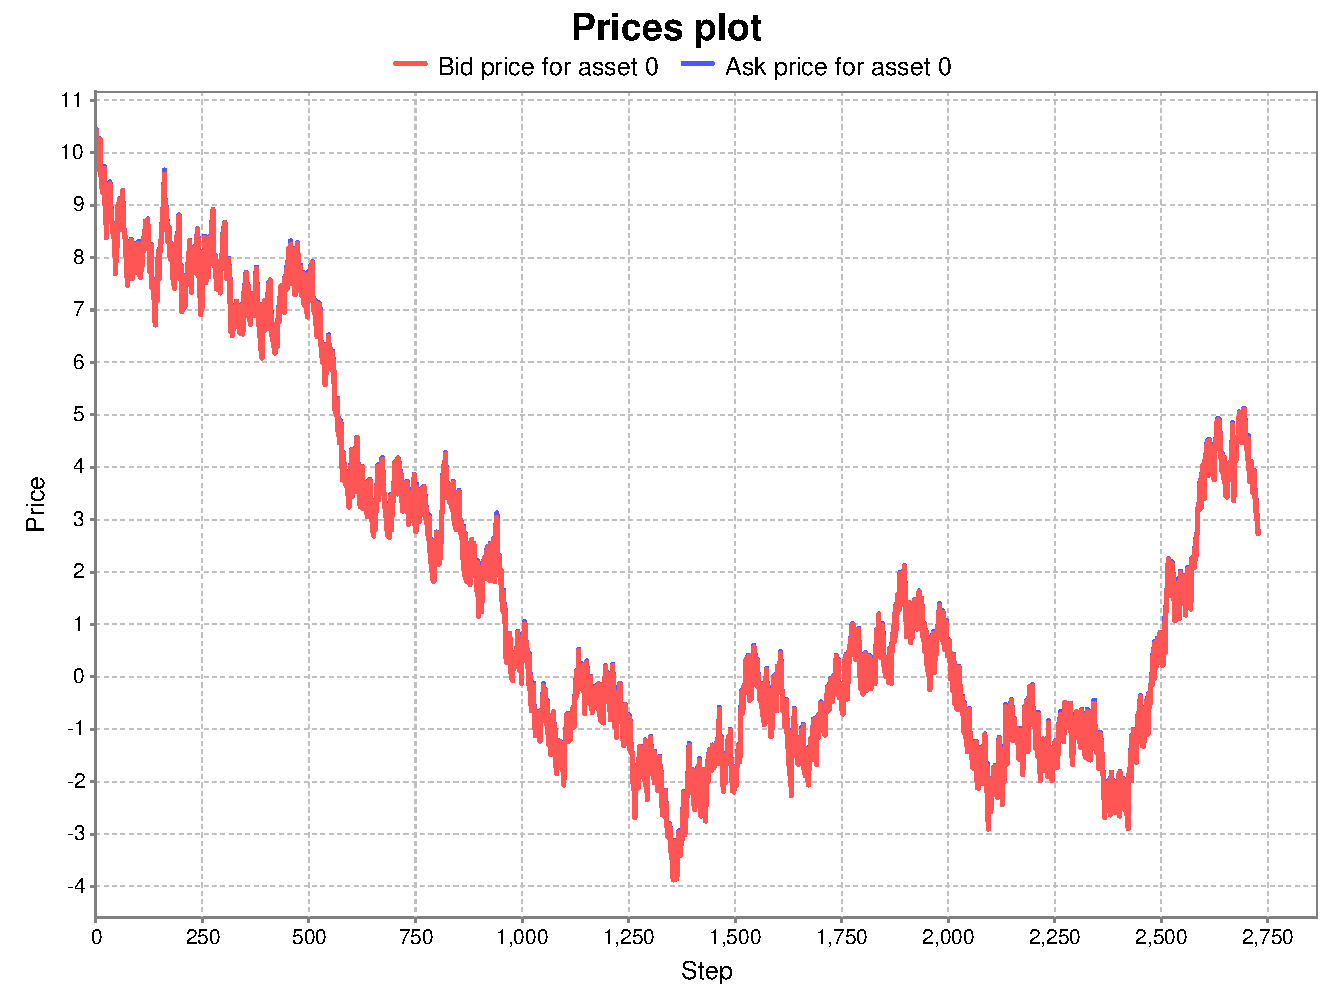
\includegraphics[width=1.0\textwidth]{../graphics/FC-pricesPlot.pdf}}} \quad
      }
    \mbox{
      \subfigure[Raw and absolute log returns.]{\scalebox{0.33}{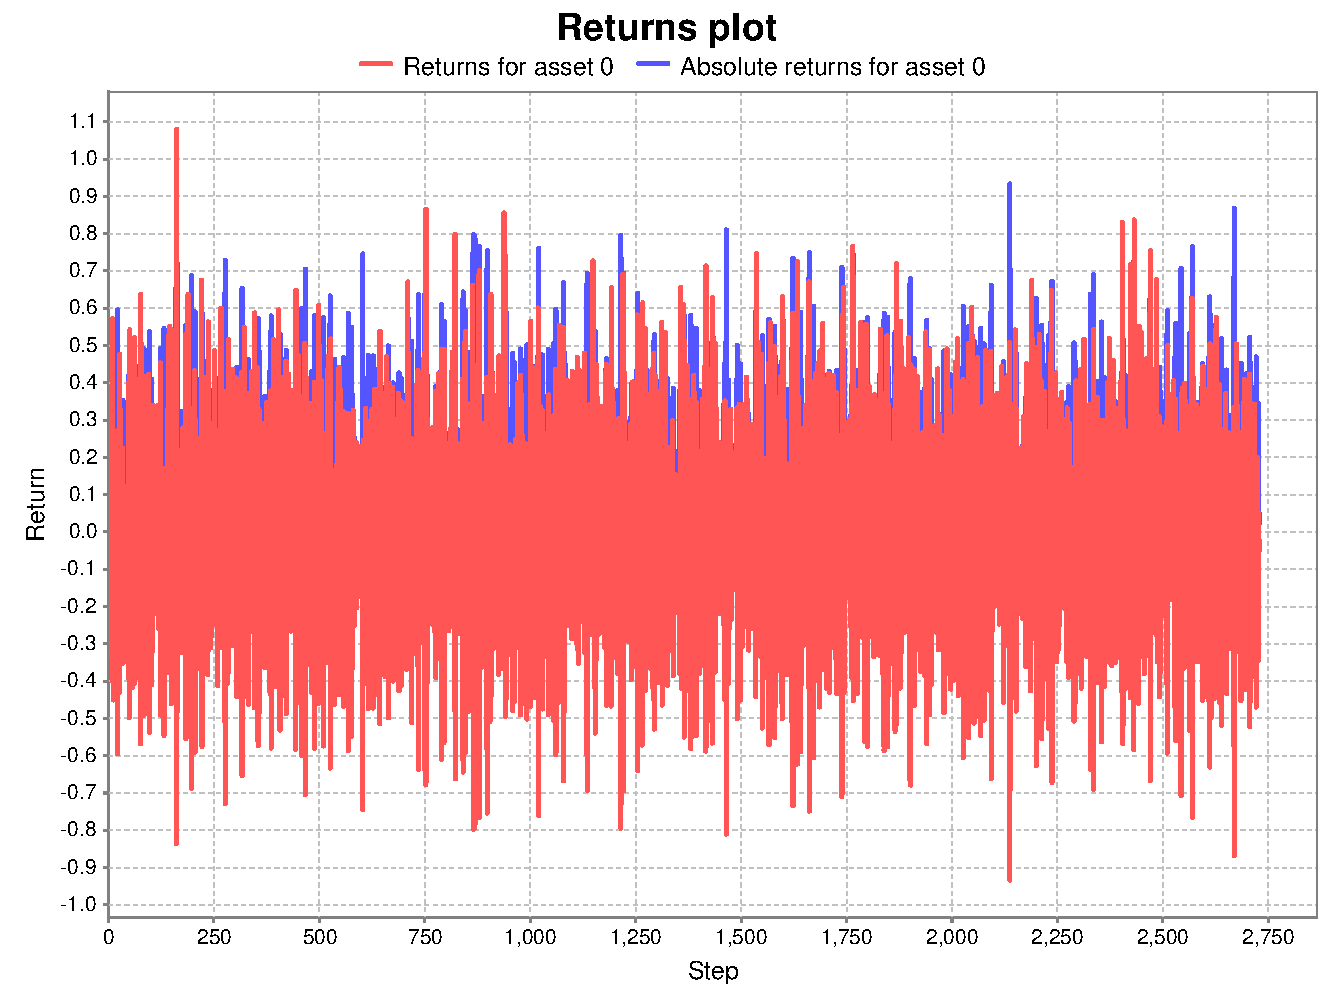
\includegraphics[width=1.00\textwidth]{../graphics/FC-returnsPlot.pdf}}}
      \quad
      \subfigure[Returns histogram.]{\scalebox{0.33}{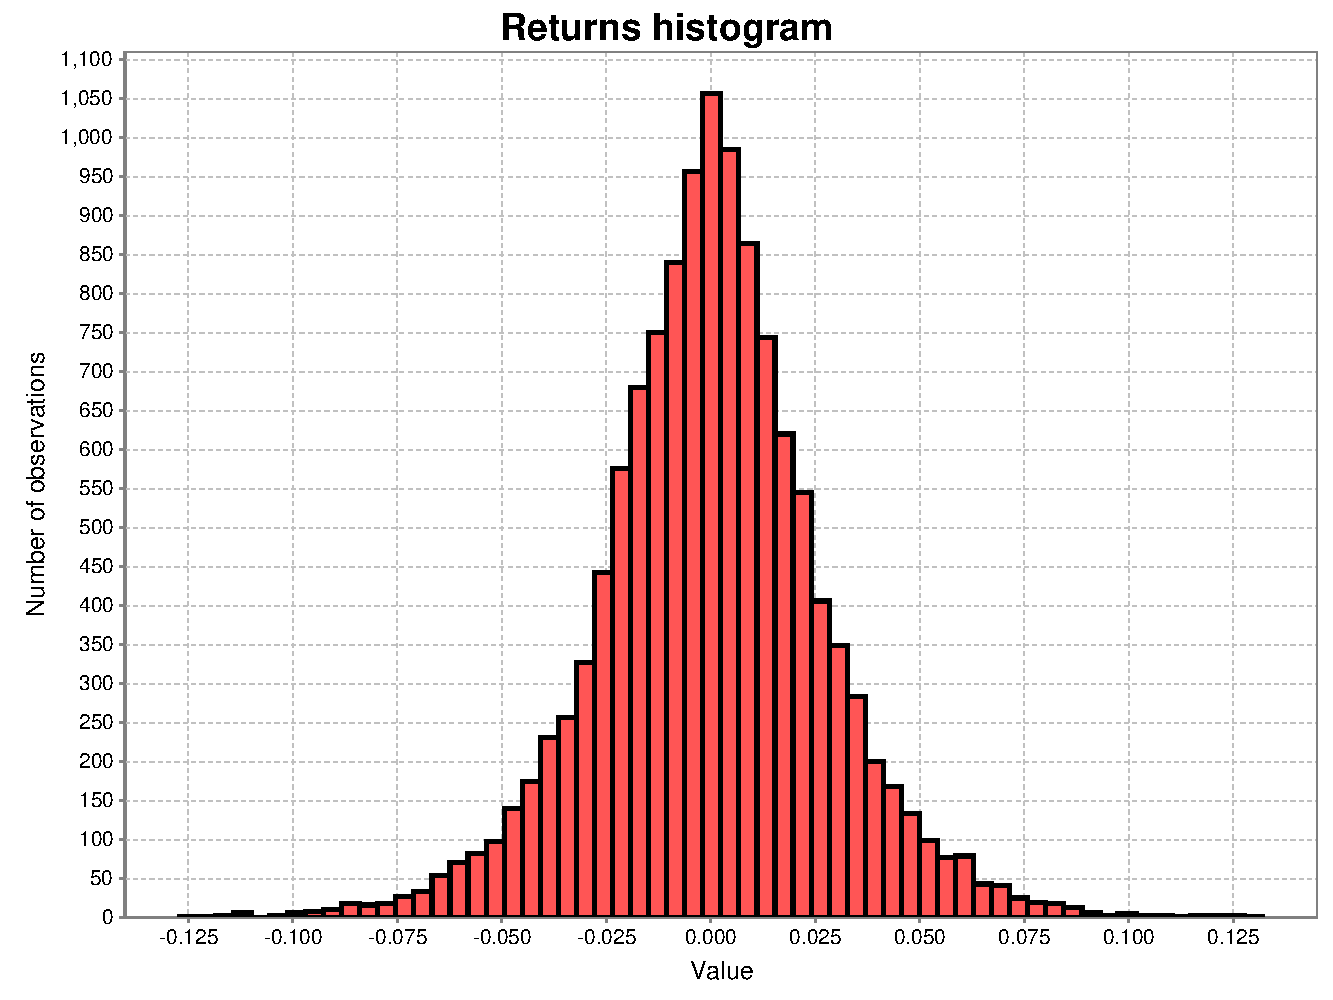
\includegraphics[width=1.00\textwidth]{../graphics/FC-returnsHistogram.pdf}}}
      \quad
      \subfigure[Returns histogram in logs.]{\scalebox{0.33}{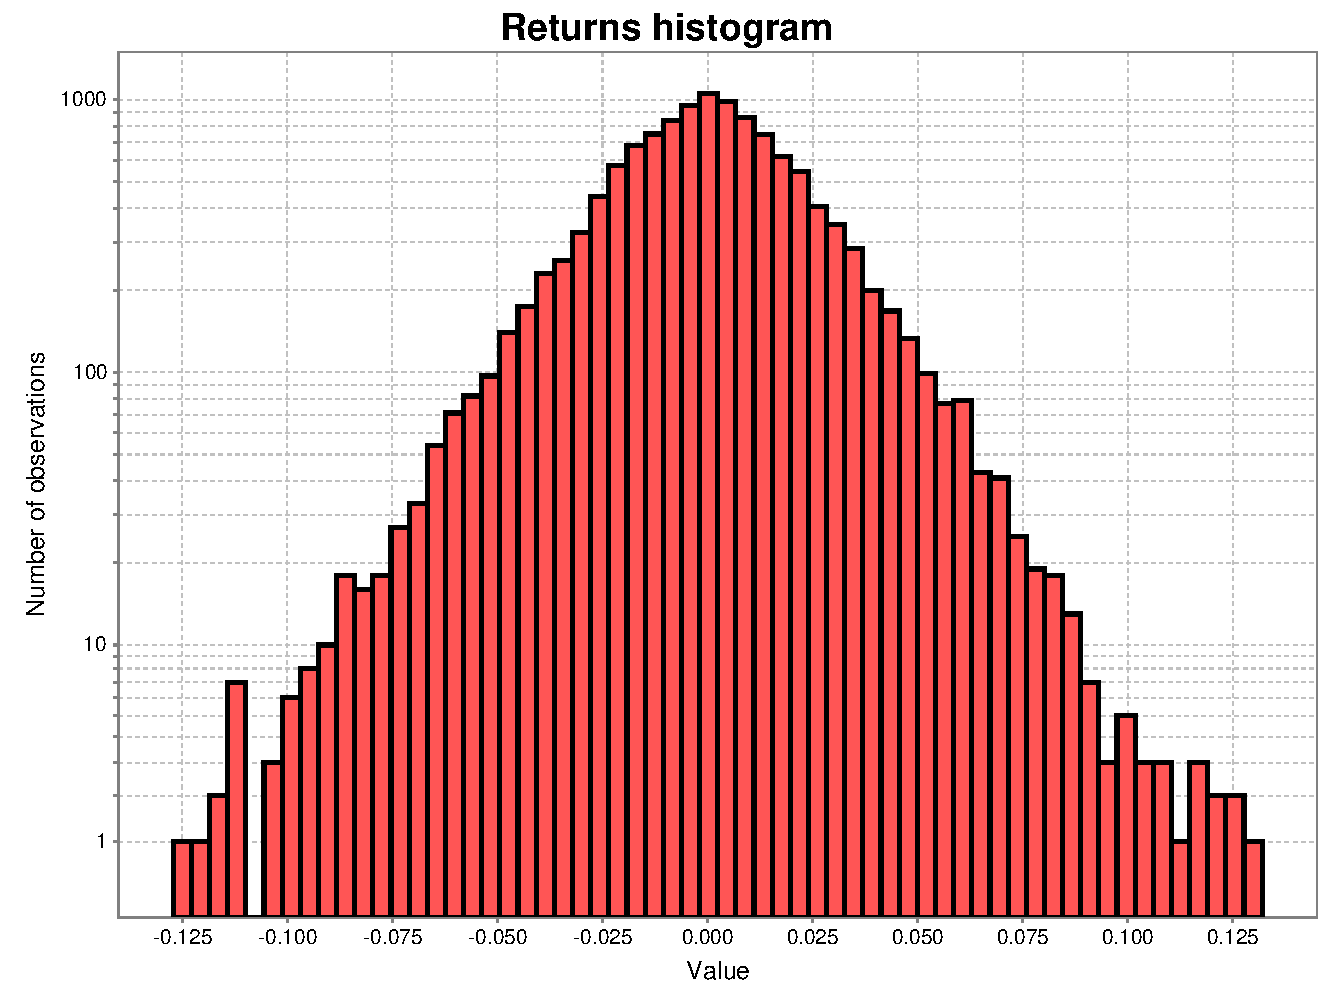
\includegraphics[width=1.00\textwidth]{../graphics/FC-logReturnsHistogram.pdf}}}       
}
    \mbox{
      \subfigure[Annualized moving average volatility]{\scalebox{0.33}{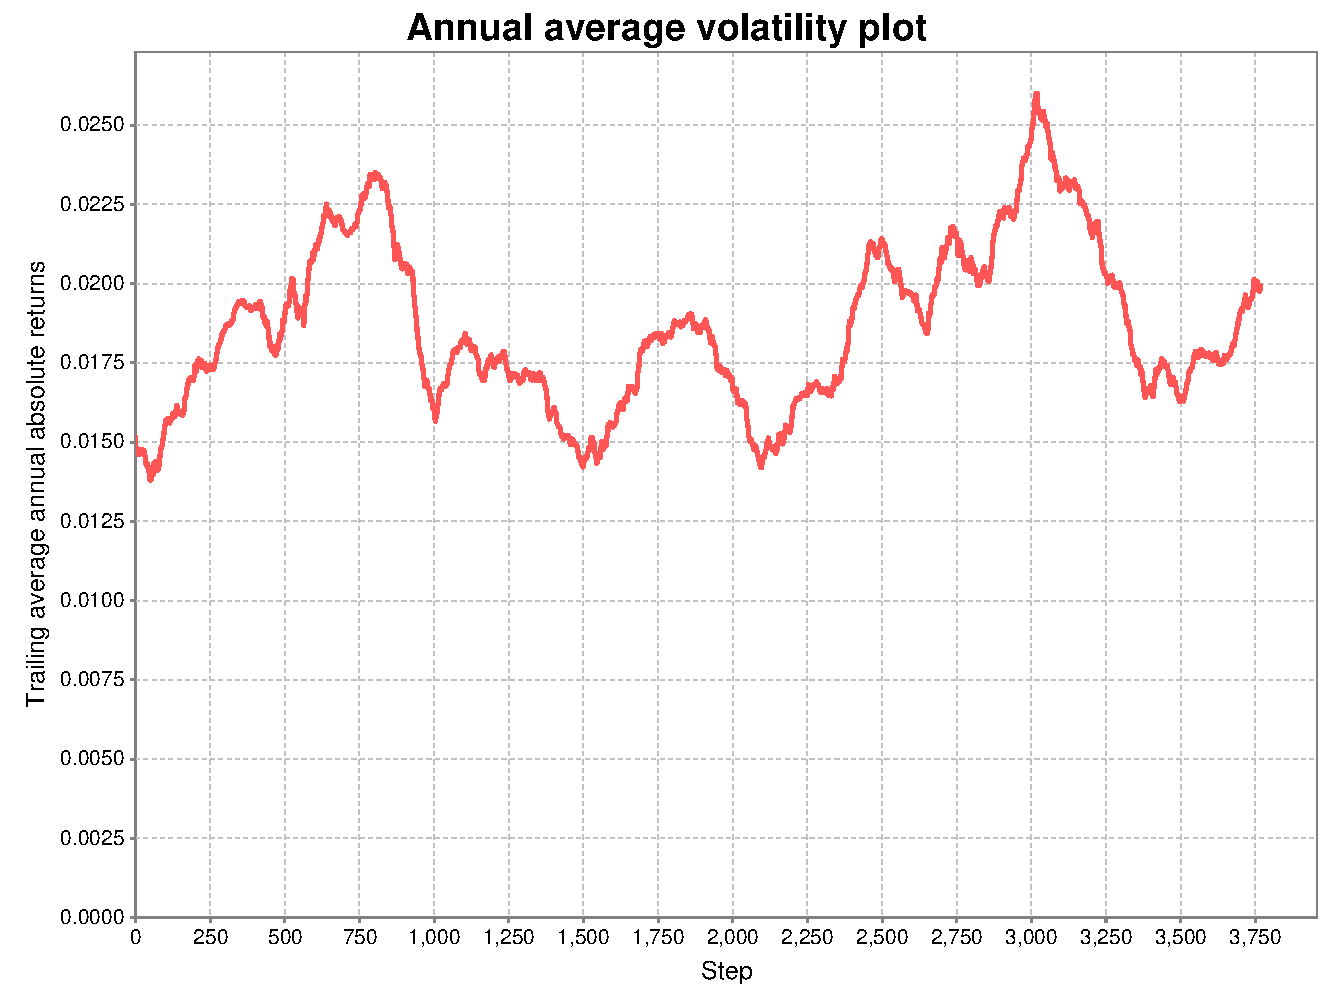
\includegraphics[width=1.00\textwidth]{../graphics/FC-avgVolatility.pdf}}}
      \quad
      \subfigure[Snapshot of orderbook.]{\scalebox{0.33}{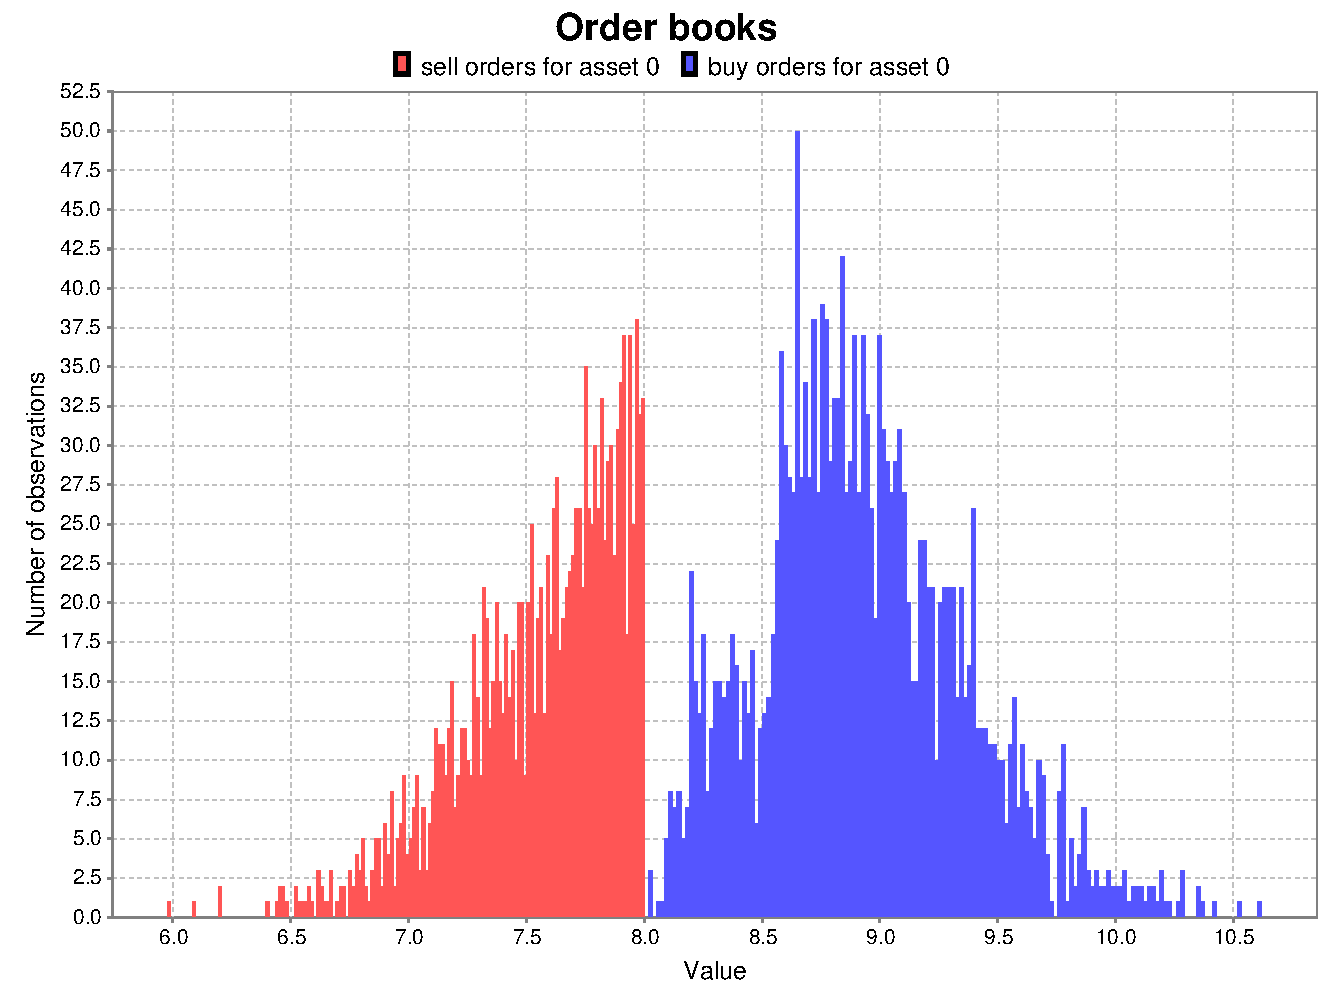
\includegraphics[width=1.00\textwidth]{../graphics/FC-orderbooks.pdf}}}
      \quad
      \subfigure[Autocorrelation of absolute returns.]{\scalebox{0.33}{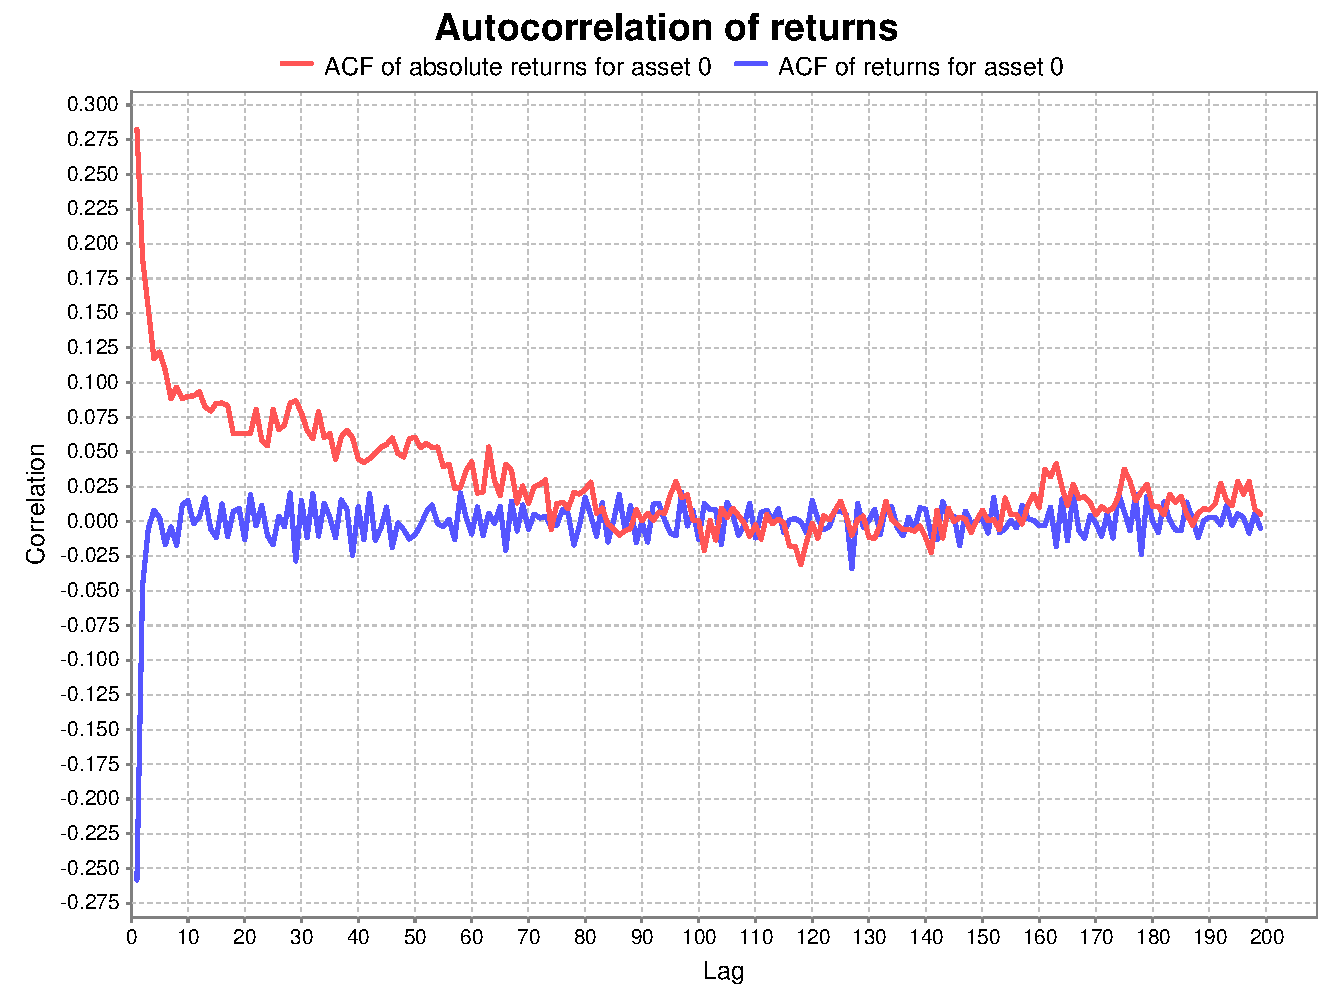
\includegraphics[width=1.00\textwidth]{../graphics/FC-acfReturns.pdf}}}
      }
    \caption{Examples of outputs and statistics from a single run of the Farmer-Cont hybryd.}
    \label{fig:ContLargeSSim}
  \end{center}
\end{figure}


TODO Show results.
TODO Note: liquidity issues



\section{Verification of Correctness}

TODO: show results side by side with original papers' figures

These compare well with data shown in the original paper (shown in Figures \ref{fig:ContSmallSPap} and \ref{fig:ContLargeSPap}).


\begin{figure}[htbp]
  \begin{center}
    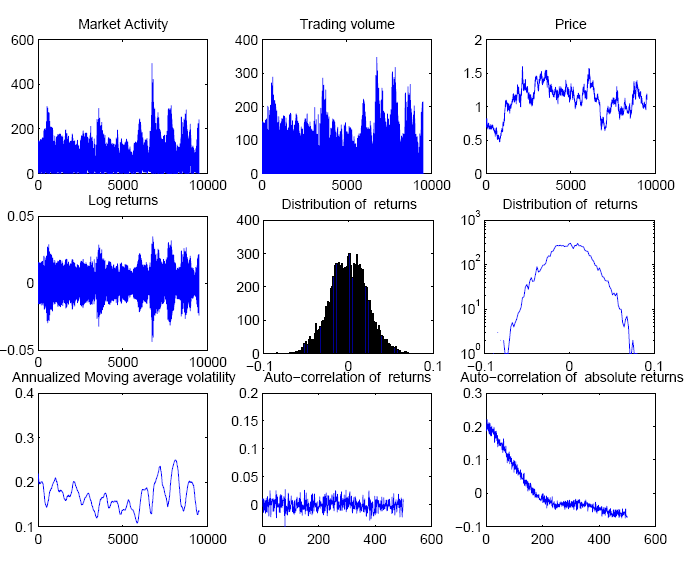
\includegraphics[width=0.8\textwidth]{../graphics/Cont-Fig3.png}
    \caption{Outputs from Cont's paper with $D=0.001$, $s=0.01$. Compare directly to Figure \ref{fig:ContSmallSSim}.}
    \label{fig:ContSmallSPap}
  \end{center}
\end{figure}

\begin{figure}[htbp]
  \begin{center}
    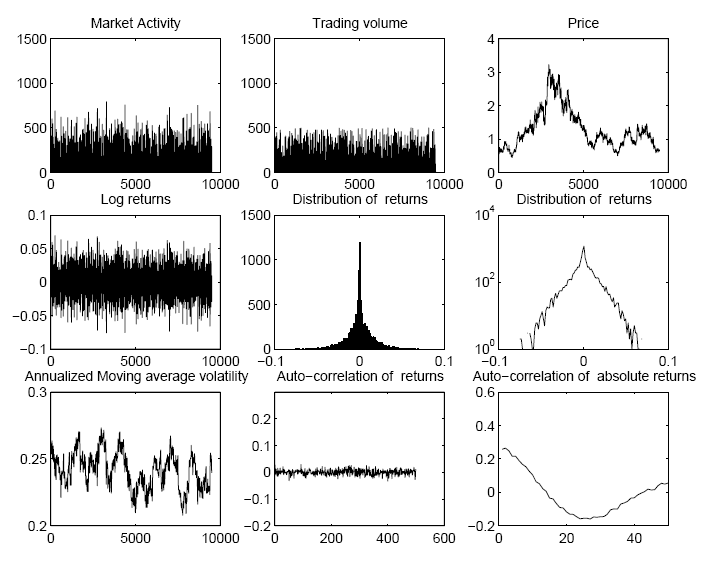
\includegraphics[width=0.8\textwidth]{../graphics/Cont-Fig4.png}
    \caption{Outputs from Cont's paper with $D=0.001$, $s=0.1$. Compare directly to Figure \ref{fig:ContLargeSSim}.}
    \label{fig:ContLargeSPap}
  \end{center}
\end{figure}

\section{Muti-run Instrumentation}

\begin{figure}[htbp]
  \begin{center}
   \mbox{
      \subfigure[Autocorrelation functions]{\scalebox{0.5}{\quad \quad 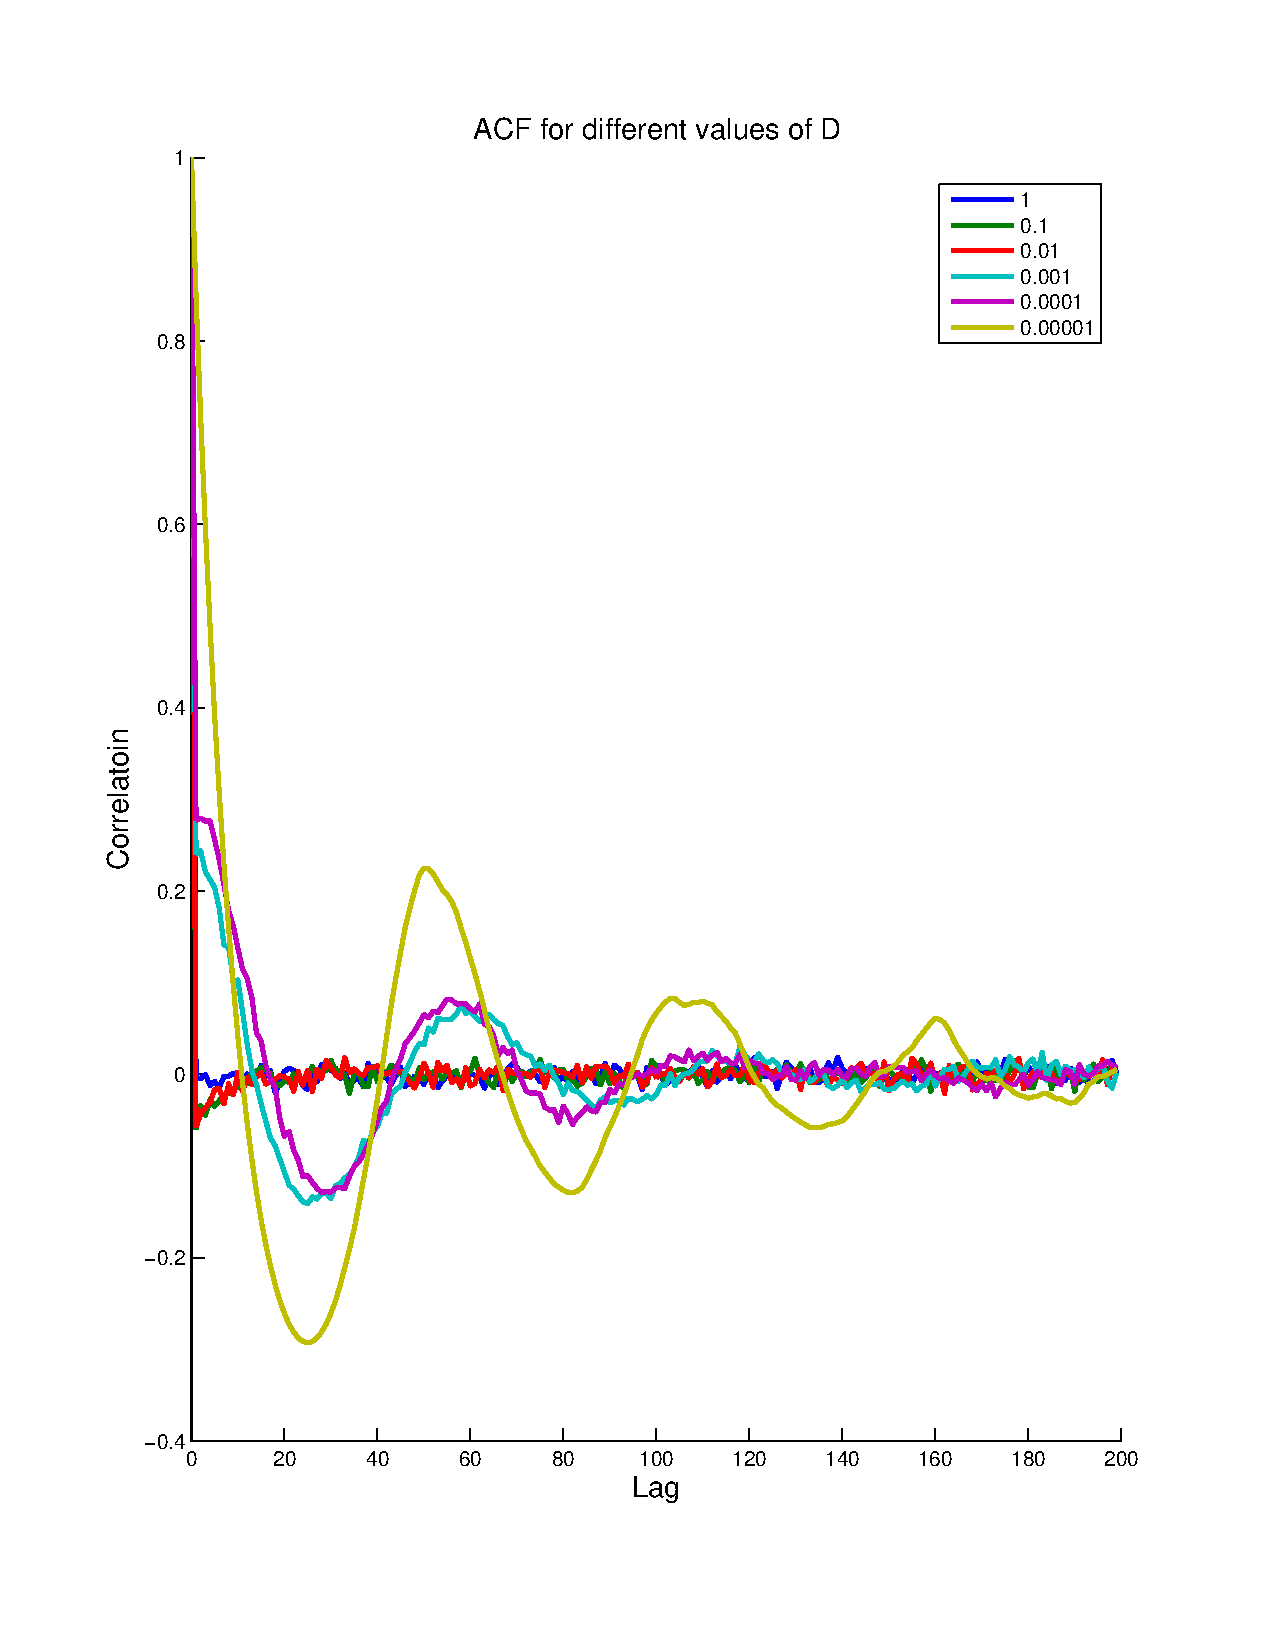
\includegraphics[width=1.0\textwidth]{../graphics/comparisonOfACFs.pdf}}} \quad
      \subfigure[Return distributions]{\scalebox{0.5}{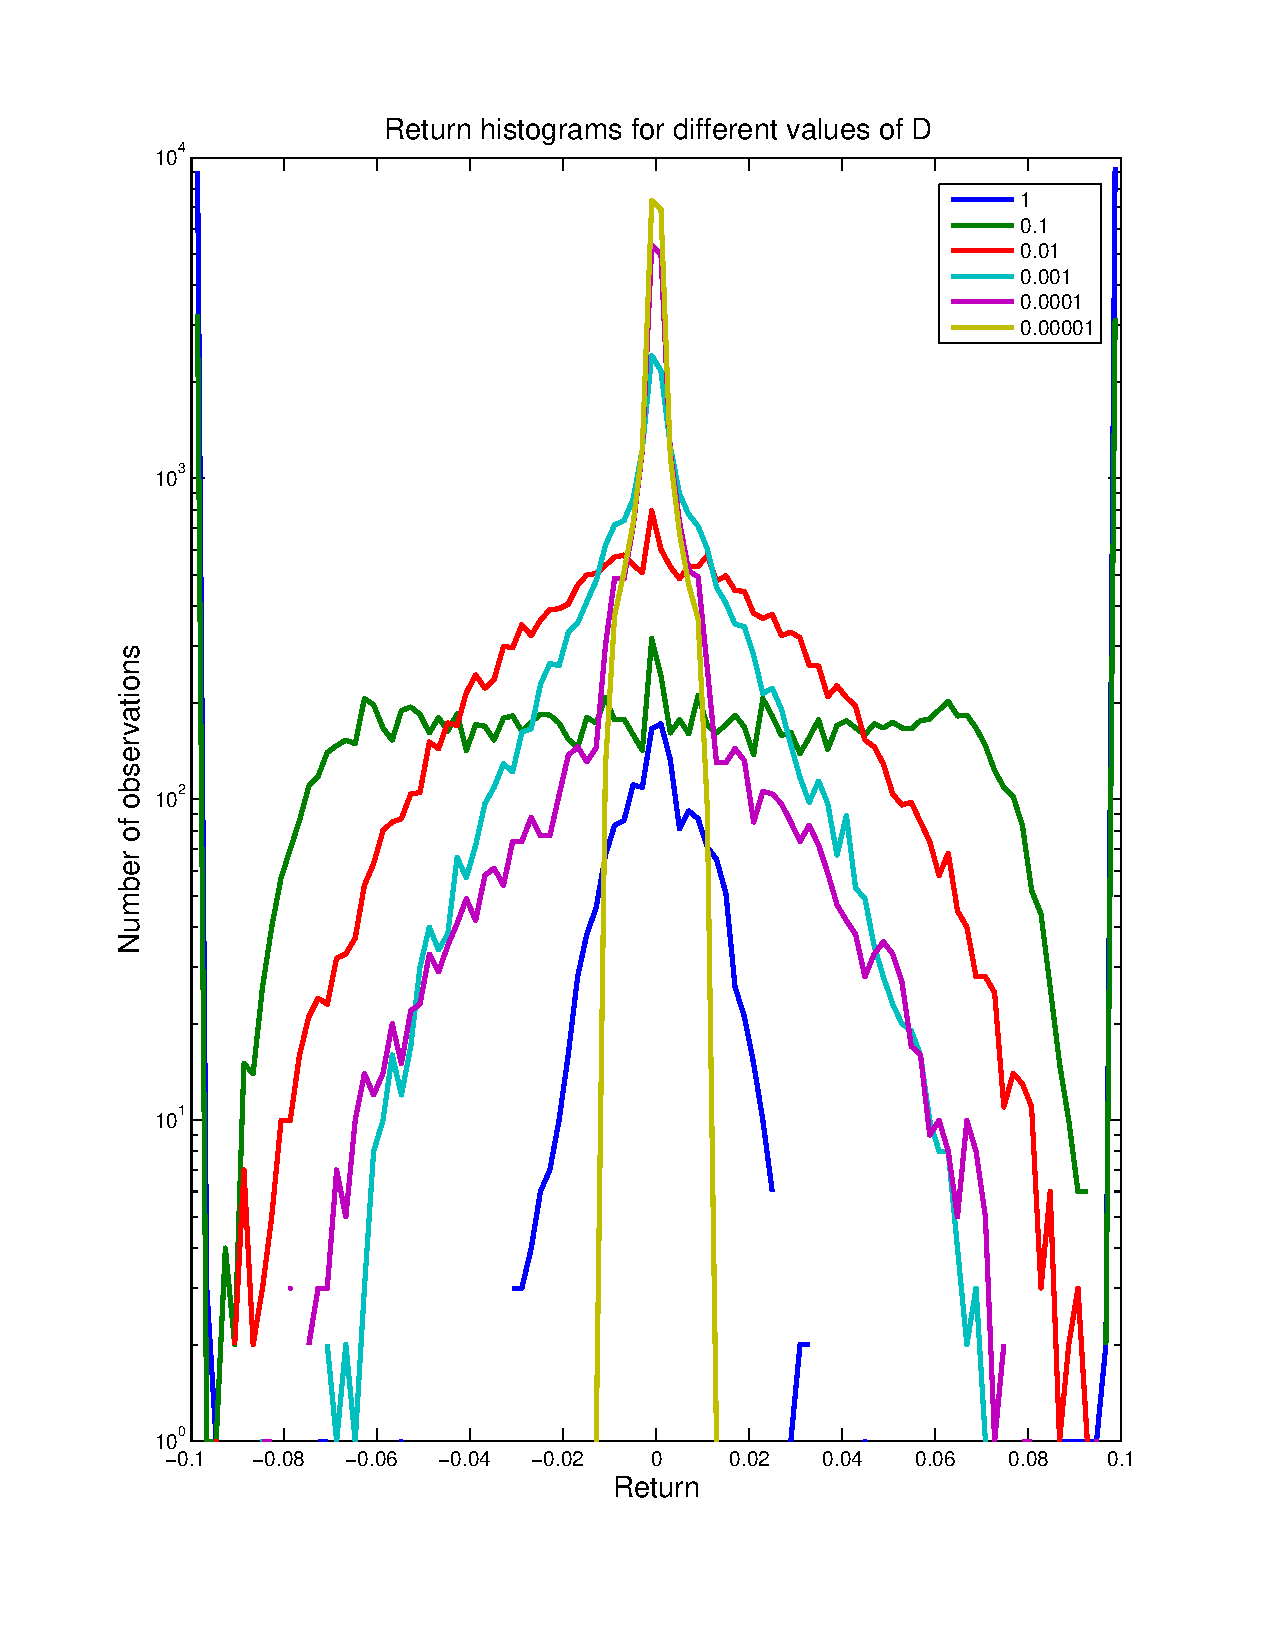
\includegraphics[width=1.00\textwidth]{../graphics/comparisonOfHistograms.pdf}}}
      }
    \caption{Autocorrelation and distributions in Cont simulation with $s=0.1$ and varying $D$, averaged over many runs.}
    \label{fig:ContMultiRun}
  \end{center}
\end{figure}

\bibliographystyle{plainnat}
\bibliography{master}

\end{document}

%%%%%%%%%%%%%%%%%%%%%%%%%%%%%%%%%%%%%%%%%%%%%%%%%%%%%%%%%%%%%%%%%%%%%%
%% The end.
%%%%%%%%%%%%%%%%%%%%%%%%%%%%%%%%%%%%%%%%%%%%%%%%%%%%%%%%%%%%%%%%%%%%%% 
